
\documentclass{lmcs}

\usepackage[T1]{fontenc}
\usepackage[utf8]{inputenc}
\usepackage{amssymb,mathtools,booktabs}
\usepackage{tikz}
\usepackage{xurl}
\microtypesetup{expansion=false}

\urlstyle{tt}
\Urlmuskip=0mu plus 2mu\relax
\DeclareUrlCommand\AgdaPath{\urlstyle{tt}}

\newcommand{\N}{\mathbb{N}}
\newcommand{\Z}{\mathbb{Z}}
\newcommand{\U}{\mathcal{U}}
\newcommand{\B}{\mathcal{B}}
\newcommand{\Lcal}{\mathcal{L}}
\newcommand{\Gcal}{\mathcal{G}}
\newcommand{\RawDecl}{\mathrm{RawDecl}}
\newcommand{\Cand}{\mathrm{Cand}}
\newcommand{\Layer}{\mathrm{Layer}}
\newcommand{\NormSig}{\mathrm{NormSig}}
\newcommand{\ObSig}{\mathrm{ObSig}}
\newcommand{\Ix}{\mathrm{Ix}}
\newcommand{\Real}{\mathrm{Real}}
\newcommand{\Prim}{\mathrm{Prim}}
\newcommand{\Der}{\mathrm{Der}}
\newcommand{\PrimClasses}{\mathrm{PrimClasses}}
\newcommand{\Foot}{\mathrm{Foot}}
\newcommand{\Shape}{\Pi_{\!\infty}}
\newcommand{\Supp}{\mathrm{Supp}}
\newcommand{\hcomp}{\mathrm{hcomp}}
\newcommand{\compop}{\mathrm{comp}}
\newcommand{\transp}{\mathrm{transp}}
\newcommand{\Fib}{\mathrm{Fib}}

\title[Primitive Trace Depth and Affine Recurrence]{Primitive Public Structural Trace Depth and Affine Recurrence in Cubical Sealed Extensions}

\author[H.\ Lande]{Halvor Lande}
\email{hsl@awc.no}

\keywords{cubical type theory, extension calculus, coherence, univalence}
\subjclass[2012]{Theory of computation~$\rightarrow$~Type theory; Mathematics of computing~$\rightarrow$~Algebraic topology}

\begin{document}

\begin{abstract}
We study admissible sealed structural extensions of cubical foundations with substitution-stable Kan composition and filling. The result is not a truncation theorem: higher cubical cells, cubes, paths, homotopies, and user-supplied higher HIT constructors may exist at every dimension, with arbitrary higher user constructors counted as payload rather than automatically generated structural trace. The theorem concerns the primitive public structural trace exported at sealed boundaries. Stated parametrically in a semantic adequacy package for a fixed raw extension calculus, it separates exact realized obligation objects $\Real_k(X)$ from the primitive public trace fields that survive in $\mu$-minimal normalized signatures. Cubical horn computation via $\hcomp$ and $\mathsf{hfill}$ gives exact stabilization $\Real_k(X)\simeq\Real_2(X)$ for $k\geq2$, derives higher structural obligations from binary boundary trace, and a swap obstruction shows that unary data do not suffice in general. A separate recent-history theorem turns the exact depth-two bound into a genuine two-layer chronological window. Consequently, under the explicit full-coupling hypothesis, primitive trace cost satisfies the payload-aware recurrence
\[
  \mu_{n+1} = \mu_n + \mu_{n-1} + \kappa_n+\kappa_{n-1}.
\]
Under the further constant-payload specialization $\kappa_n=c$, the shifted sequence $U_n=\mu_n+2c$ is Fibonacci. The accompanying Cubical Agda development formalizes the candidate-and-obligation calculus, the fixed raw bridge to canonical trace signatures, active-basis naturality, sparse/full recurrence, and the case-study audit; \autoref{sec:mechanization} records the paper-to-Agda map and the trusted boundary.
\end{abstract}

\maketitle

\section{Introduction}
\label{sec:introduction}

\subsection{The metatheoretic question}

This paper concerns a simple but surprisingly rigid question.

\begin{quote}
When a type-theoretic core calculus is extended by sealing a new structure against the existing interface, how does the cost of integration scale with the historical depth of the library?
\end{quote}

The question is not about transparent user developments inside a fixed library. It is about \emph{sealed} extensions: new type formers, modalities, or promoted interface packages whose public behavior becomes part of the global exported interface. More specifically, the paper studies the worst-case regime of \emph{foundational core extensions}: globally acting additions whose exported payload must be specified across the currently active interface. Examples include extending a univalent universe hierarchy, where the decoding machinery must be updated against the library's active codes; adding a global modality presented by explicit modal dependent-type syntax, such as a Fitch-style dependent right adjoint or its cubical multimodal refinements~\cite{birkedal-modal-dtt,aagaard-cubical-mtt}, whose action must distribute across the exported type formers and transports already present; and heavily promoted generic interfaces whose action is intended to range over the whole library. In that setting, extension is constrained not only by local typing rules, but also by the obligation to interact coherently with the eliminators, transports, computation principles, and comparison data already exported by the library.

Orthogonal extensions are not the subject of this recurrence law. Adjoining a new datatype such as \texttt{Tree} to a library that already contains \texttt{List} and \texttt{Socket} need not introduce primitive \texttt{Tree}--\texttt{Socket} interaction data merely to preserve canonicity. Such sparse or local extensions are important in practice, but they do not exhibit the maximal coupling pattern that this paper isolates. Ordinary user-level library growth therefore forms a sparse dependency DAG in general; the recurrence theorem studies only the asymptotic foundational-core regime of monolithic, globally acting extensions.

The central observation is that these obligations are stratified by historical depth. Some are purely unary: the new layer must act on one previously exported generator. Others are genuinely binary: the new layer must preserve a previously exported compatibility witness between two generators. The paper therefore tracks two related depth notions: one for exact stabilization of realized obligation objects and one for what survives in normalized public signatures.

\subsection{The theorem object and adequacy boundary}

The paper-facing theorem is parameterized by a semantic cubical foundation~$F$ and an adequacy package~$A$ that interprets admissible sealed structural extensions of~$F$ in the raw extension calculus used below. In the Agda roadmap these are the records \AgdaPath{SemanticCubicalFoundation} and \AgdaPath{RawAdequacyPackage}. The foundation supplies an interval with endpoints, cofibrations or face conditions, partial elements, path or interval-indexed equality, transport, homogeneous composition, filling, boundary laws, and substitution stability; the lower-bound witness additionally uses univalence. The adequacy package is the bridge that preserves semantic interpretation, historical support, primitive-versus-derived trace status, and exported cardinality when a semantic sealed extension is represented by raw declarations and normalized signatures.

The mechanized instance fixes one cubical object theory from the start. Let $C$ be a CCHM-style cubical core calculus with univalence and Kan composition~\cite{cubical,cchm-hits}. Over~$C$ we study a language of globally acting extensions exported through opaque public signatures. A sealing step exposes only the normalized payload and trace fields of that public signature; the internal derivation that discharged the obligations is hidden behind opacity. The recurrence law proved below is therefore an instantiated theorem about this fixed cubical extension calculus, plus the explicit raw adequacy bridge of \autoref{sec:bridge}; it is not a blanket transfer theorem for every system that carries the label ``cubical.'' Cubical Agda enters in two roles only: as a mechanization environment and as a source of native cubical constructions used to witness the lower-bound phenomena.

\subsection{What is not claimed}

The theorem is deliberately narrower than several nearby slogans. It is not a theorem about arbitrary Cubical Agda programs, and it does not model transparent user-level library growth. It is not a theorem about every cubical type theory or about plain HoTT without the cubical horn-computation package isolated later in the paper. It does not say that arbitrary higher HoTT filler spaces are contractible; the contractible factors below are structural horn-extension packages produced by the fixed sealing calculus. Finally, the quantity~$\mu$ is not a source-code line count. It counts primitive public trace schemas after normalization and opacity, so refactorings that preserve the sealed public interface do not change it.

\begin{table}[t]
\centering
\caption{Scope at a glance.}
\label{tab:scope-at-glance}
\small
\begin{tabular}{@{}p{0.44\linewidth}p{0.44\linewidth}@{}}
\toprule
In scope & Out of scope \\
\midrule
Admissible sealed structural extensions & Ordinary transparent definitions and lemmas \\
Primitive public structural trace at sealed boundaries & Arbitrary user payload, including higher HIT constructors \\
Higher structural obligations derived from binary trace by Kan composition and filling & A claim that higher cubical objects or paths vanish \\
Full-coupling recurrence equality & Sparse or orthogonal growth as Fibonacci equality \\
The fixed raw adequacy bridge recorded in \autoref{sec:bridge} & A parser or elaborator adequacy theorem for arbitrary Cubical Agda programs \\
\bottomrule
\end{tabular}
\end{table}

\subsection{The core thesis}

The exact metatheoretic invariant is the \emph{obligation depth}~$d_{\mathrm{obl}}$; the separate surface-syntactic invariant is the \emph{minimal-signature depth}~$d_\mu$. The thesis of the paper is that, once obligation depth is isolated from minimal-signature elimination, the asymptotic law of integration becomes forced.

\begin{quote}
In the fixed fully coupled cubical extension calculus of this paper, primitive public structural trace obeys a depth-two affine recurrence; under uniform payload size, the shifted sequence is Fibonacci.
\end{quote}

Here ``fully coupled'' refers only to the foundational-core regime just described: admissible extensions are globally acting payloads whose semantics or promoted action is intended to range over the whole active interface, not orthogonal additions that leave most earlier exports untouched. Within that regime, the operative assumption is the scope of the advertised global action, not a prior density axiom. \autoref{thm:canonicity} identifies the primitive active \emph{basis} interface of this fixed extension calculus: native core extensions are constrained by canonicity-preserving totality of the operational semantics, while promoted interface packages are constrained by operational exhaustiveness of the exported global interface. The resulting recurrence is stated over the presentation-invariant minimal opaque cost~$\mu$, not over a chosen surface presentation. In extensional systems with UIP, the obligation depth collapses to~$1$, and under uniform payload size the recurrence is first-order affine. In the fixed cubical extension calculus studied here, the obligation depth is~$2$, and \autoref{thm:higher-elim} gives the separate surface-syntactic bound $d_\mu \leq 2$; after the constant-payload shift the affine law becomes Fibonacci.

\begin{quote}
\textbf{Main theorem at a glance.}
Let $F$ be a cubical foundation with substitution-stable Kan composition and filling, and let $A$ be an adequacy package for admissible sealed structural extensions of~$F$. The primitive public structural trace has exact coherence depth~$2$: higher structural integration obligations are derived from binary boundary trace by the Kan structure, while the swap obstruction shows that unary trace alone is insufficient. Instantiating $F$ and~$A$ with the fixed CCHM-style core~$C$ and the raw bridge of \autoref{sec:bridge}, surviving primitive support has a two-layer chronological window.

For a fully coupled sequence of sealed extensions in that instantiated setting, the primitive trace cost satisfies
\[
  \mu_{n+1} = \mu_n + \mu_{n-1} + \kappa_n + \kappa_{n-1}.
\]
Under the additional constant payload assumption $\kappa_n=c$, this specializes to the shifted Fibonacci recurrence of \autoref{cor:fibonacci}. Sparse and orthogonal footprints remain bounded or sparse regimes, not equality-style Fibonacci laws.
\end{quote}

\begin{quote}
\small
\textbf{Frequently confused distinctions.}
The exact realized obligation object $\Real_k(X)$ is not the primitive public
trace signature counted by~$\mu$. A contractible exact horn factor is not an
absent obligation; it is present in $\Real_k(X)$ but contributes no primitive
field after canonical replacement. A derived trace field is not counted as a
primitive one. An arity bound is not yet a chronological window; the
recent-history theorem supplies that extra fact. Finally, a sparse dependency
footprint is not the fully coupled footprint used in the recurrence.
\end{quote}

\subsection{Summary of contributions}

The paper develops one theorem package with three main components. The
dependency table below is the canonical short summary of how these components
fit together; later sections prove the entries rather than restating the whole
stack.

\begin{enumerate}
\item We define the sealed extension calculus, its raw declarations, admissibility
judgments, normalized public signatures, primitive/derived tags, support, and
fully coupled active footprints. Counts are taken on canonical normal forms, so
record rebundling, currying, transparent aliases, and shell splitting do not
change the measured interface.
\item We separate exact realized obligation objects from $\mu$-minimal public
trace signatures. The cubical theorem proves depth-two exact stabilization,
eliminates higher primitive trace fields from minimal public form, supplies a
two-layer chronological window for surviving binary fields, and gives explicit
binary lower-bound witnesses.
\item We combine the trace principle with the chronological-window theorem to
obtain a sparse footprint recurrence and its fully coupled affine endpoint. Under
constant payload size~$c$, the depth-two cubical case specializes to
    \[
      \mu_{n+1} = \mu_n + \mu_{n-1} + 2c,
    \]
    and the shifted sequence $U_n=\mu_n+2c$ is Fibonacci. The associated structural inflation factor still converges to the Golden Ratio.
\end{enumerate}

\autoref{sec:mechanization} records the exact paper-to-Agda map and the trusted
boundary. Its purpose is to audit the theorem package once, not to replace the
mathematical statements in the body with a second copy of the same list.

\paragraph{Claim discipline.}
Every theorem-level assertion made in the introduction is discharged later at
its declared level: fixed raw syntax and admissibility in
\autoref{sec:framework} and \autoref{sec:bridge}, exact realized-object
stabilization in \autoref{thm:upper} and \autoref{cor:contractible-factor},
minimal public-signature elimination in \autoref{thm:higher-elim}, chronological
support in \autoref{lem:telescopic} and \autoref{cor:chrono-window}, binary
necessity in \autoref{thm:adjunction}, and the affine recurrence in
\autoref{thm:recurrence}. Broader examples in the opening paragraphs are used
only as motivating instances of globally acting sealed extensions unless they
are separately named as theorem-level examples.

\autoref{tab:claim-map} summarizes the dependency architecture that the rest of the paper keeps separate: exact stabilization of realized obligation objects, elimination from $\mu$-minimal signatures, recent-history factorization, lower-bound binary obstructions, the affine recurrence itself, and the status of each layer in the mechanization.

\begin{table}[t]
\centering
\caption{Dependency map of the depth-two theorem stack.}
\label{tab:claim-map}
\small
\begin{tabular}{@{}p{0.19\linewidth}p{0.26\linewidth}p{0.32\linewidth}p{0.13\linewidth}@{}}
\toprule
Claim & Logical role & Main inputs & Status \\
\midrule
\autoref{thm:upper}, \autoref{cor:contractible-factor} & exact $\Real$-stabilization at depth~$2$ and trivialization of higher exact fibers & horn-reduction metatheory and contractibility of cubical horn-extension fibers & fully formalized \\
\autoref{thm:higher-elim} & elimination from $\mu$-minimal normalized public signatures & \autoref{lem:horn-reduction}, \autoref{thm:computational-replacement}, canonical presentation, and the fixed raw bridge & formalized with bridge \\
\autoref{lem:telescopic} & recent-history factorization of surviving binary primitive fields & factorization-complete trace export, the formal chronological-window chain, and the fixed raw bridge & formalized with bridge \\
\autoref{thm:adjunction}, \autoref{thm:clutching} & lower-bound binary obstruction & swap barrier, adjunction coherence, and clutching-family witness & fully formalized \\
\autoref{thm:recurrence} & affine recurrence for $\mu$ & \autoref{thm:trace}, \autoref{cor:mu-delta}, the sparse/full recurrence package, and the chronological-window package & formalized with bridge \\
\autoref{sec:mechanization} & trusted-boundary audit & theorem-to-Agda correspondence for all rows above & mixed; see \autoref{tab:mechanization-status} \\
\bottomrule
\end{tabular}
\end{table}

\begin{figure}[t]
\centering
\[
\begin{array}{c}
\Real_k(X)\simeq\Real_2(X)
\\
\text{exact obligation objects}
\\[0.8ex]
\downarrow\ \text{canonical replacement}
\\[0.8ex]
d_\mu\leq 2
\\
\mu\text{-minimal public signatures}
\\[0.8ex]
\downarrow\ \text{recent-history factorization}
\\[0.8ex]
\Foot_n^{(2)}
\\
\text{two-layer primitive support}
\\[0.8ex]
\downarrow\ \text{full coupling}
\\[0.8ex]
\mu_{n+1}=\mu_n+\mu_{n-1}+\kappa_n+\kappa_{n-1}.
\end{array}
\]
\caption{Dependency graph for the main theorem package. Exact stabilization is a statement about realized obligation objects. Canonical replacement turns higher horn factors into derived trace fields in $\mu$-minimal public signatures. Recent-history factorization gives a two-layer primitive-support window, and the full-coupling endpoint converts that window into the affine recurrence.}
\label{fig:dependency-graph}
\end{figure}

\subsection{Related work}
\label{sec:related}

The higher-dimensional background comes from the interpretation of intensional
identity types as weak $\omega$-groupoids, developed by Lumsdaine~\cite{lumsdaine}
and van den Berg and Garner~\cite{vdberg-garner}. The operational substrate used
here is the CCHM-style cubical core of Cohen, Coquand, Huber, and
M\"ortberg~\cite{cubical}, together with higher inductive types and Kan
composition~\cite{cchm-hits}. Cubical Agda~\cite{cubical-agda} provides the proof
assistant environment and the native cubical programs used in the development,
but the theorem target is the sealed extension calculus defined below, not the
full Agda surface language.

Univalence is used as a source of binary obstruction examples: equivalences such
as the boolean swap produce paths along which unary objectwise action data must
be transported coherently. For modal and mixed-equality examples we use explicit
type-theoretic syntax rather than informal endofunctor language. Dependent right
adjoints give a Fitch-style dependent presentation~\cite{birkedal-modal-dtt},
cubical multimodal type theory shows how such modalities interact with cubical
structure~\cite{aagaard-cubical-mtt}, and two-level type theories provide the
comparison point for mixed weak/strict equality foundations~\cite{altenkirch-strict,annenkov-2ltt}.

The coherence-theoretic side is informed by Mac Lane's coherence
theorem~\cite{maclane-coherence}, Stasheff's analysis of higher
associativity~\cite{stasheff}, and the well-foundedness approach to coherence of
Kraus and von Raumer~\cite{kraus-vonraumer}. Our contribution is not a replacement
for those qualitative coherence results. It is a normalized cost invariant for
sealed globally acting extensions: the counted object is the primitive opaque
trace interface that remains after canonical presentation and opacity.

The closest programming-language analogy is not source size, but normalized
interfaces for algebraic signatures and module systems. The paper counts the
public primitive schema boundary after transparent definitions, aliases, and
presentation artifacts have been quotiented away. The topological family used for
the lower bound is the classical clutching description of principal bundles over
spheres; for standard bundle-theoretic background we refer to
Husemoller~\cite{husemoller}. The univalent and cubical perspective sits in the
general landscape of homotopy type theory and univalent foundations~\cite{hott}.

\section{A fixed cubical extension calculus}
\label{sec:framework}

We fix throughout a cubical extension calculus built over a chosen CCHM-style core~$C$ with univalence and Kan composition. Its admissible extensions are globally acting payloads exported through opaque public signatures, and later layers may depend only on that public interface. The library therefore grows as a sequence
\[
  \B_0 \leadsto \B_1 \leadsto \B_2 \leadsto \cdots
\]
of states, where each step adjoins one new sealed layer of the fixed extension calculus.

\subsection{Raw syntax and judgments}
\label{subsec:raw-syntax}

The theorem target is the following raw extension calculus. Its grammar is deliberately small:
\[
\begin{array}{rcl}
  i,j,n &\in& \mathsf{LayerId},\\
  \B   &::=& \cdot \mid \B,L_i,\\
  e    &::=& (\Gamma_{\mathrm{new}},\Gamma_{\mathrm{act}},\Gamma_{\mathrm{cmp}},\sigma).
\end{array}
\]
Here $\Gamma_{\mathrm{new}}$ is the payload telescope, $\Gamma_{\mathrm{act}}$ is the telescope of unary action clauses against the selected active footprint, $\Gamma_{\mathrm{cmp}}$ is the telescope of comparison, transport, and horn-boundary clauses, and $\sigma$ is the export selection for the sealed public interface. The fixed calculus is specified by the judgments
\[
\begin{array}{rcl}
  \B\ \mathsf{wf} && \text{well-formed states},\\
  \B \vdash e : \RawDecl && \text{raw declarations},\\
  \B \vdash e\ \mathsf{adm} && \text{admissible declarations},\\
  \B \vdash \mathsf{Elab}(e) : \Cand && \text{elaboration to candidates},\\
  \B \vdash \mathsf{Seal}(e) : \Layer && \text{opaque sealing},\\
  \B \vdash N(e) : \NormSig && \text{normalized public signatures},\\
  \B \vdash \phi\ \mathsf{primitive} && \text{primitive public fields},\\
  \B \vdash \phi\ \mathsf{derived} && \text{transparent or computed fields},\\
  \B \vdash \Supp(\phi)=S && \text{historical support of a field}.
\end{array}
\]
An admissible declaration is therefore not merely a syntactic quadruple: it is a raw declaration whose payload, action clauses, comparison clauses, and export selection type-check, cover the required footprint for the declared coupling mode, and normalize to an opaque public signature. A declaration is outside the theorem target if it uses forms not generated by this grammar, relies on hidden derivations after sealing, omits required full-footprint clauses while advertising itself as fully coupled, or asks for a general Cubical Agda elaboration theorem rather than the fixed bridge of \autoref{sec:bridge}.

\begin{defi}[Raw structural clause classes]
\label{def:raw-structural-clauses}
The raw calculus uses three theorem-facing clause classes. A \emph{raw action
clause} is a field of $\Gamma_{\mathrm{act}}$ whose support mentions one prior
opaque interface site and specifies the new payload's unary action on that site.
A \emph{raw comparison clause} is a field of $\Gamma_{\mathrm{cmp}}$ whose
support mentions two prior interface sites and compares the two induced unary
composites, including transport or naturality squares. A \emph{raw horn clause}
is a field of $\Gamma_{\mathrm{cmp}}$ whose type presents a higher structural
boundary together with the missing-face/filler package of
\autoref{def:horn-extension-package}. Raw horn clauses may occur in the exact
realized obligation object, but after adequacy and computational replacement
they are classified as derived trace whenever their witness is synthesized by
the cubical Kan operations from the lower boundary.
\end{defi}

\subsection{States, extensions, and promoted packages}

\begin{defi}[State]
\label{def:state}
A \emph{state} or \emph{library} is a monotone context $\B$ closed under derivability. An evolution step
\[
  \B_n \leadsto \B_{n+1}
\]
adjoins one sealed integration layer, denoted $L_{n+1}$.
\end{defi}

\begin{defi}[Surface extensions]
\label{def:surface-extension}
Over a state~$\B_n$, a \emph{surface extension declaration} is a finite quadruple
\[
  e = (\Gamma_{\mathrm{new}}, \Gamma_{\mathrm{act}}, \Gamma_{\mathrm{cmp}}, \sigma),
\]
where $\Gamma_{\mathrm{new}}$ is a telescope of newly declared payload symbols, $\Gamma_{\mathrm{act}}$ is a finite family of unary action clauses against the active interface, $\Gamma_{\mathrm{cmp}}$ is a finite family of comparison or transport clauses, and $\sigma$ specifies which elaborated fields are exported through the sealed public interface. The admissible extensions studied in this paper are exactly those declarations whose intended action is global on the designated active interface footprint.
\end{defi}

This is a fixed raw extension calculus, not the full surface language of Cubical Agda. The mechanized bridge checks the raw declaration forms just listed and their admissibility/classification judgments; it does not claim to parse or elaborate arbitrary Agda programs.

\begin{defi}[Elaboration, sealing, and normalized public signature]
\label{def:elaboration}
Each admissible surface extension declaration~$e$ over~$\B_n$ elaborates to a core object
\[
  \mathsf{Elab}(e)
\]
of the fixed cubical core~$C$: the payload telescope elaborates to new core declarations, the action and comparison clauses elaborate to fields witnessing interaction with the active interface, and the opacity component~$\sigma$ selects the public telescope exported after sealing. The \emph{normalized public signature} of~$e$ is the counting normal form
\[
  N(e) := N(\mathsf{Elab}(e)),
\]
obtained by flattening the public telescope and discarding fields uniformly synthesized by definitional equality or the generic structural operations of the ambient cubical calculus.
\end{defi}

\begin{defi}[Presentation equivalence and minimal opaque cost]
\label{def:mu}
Two admissible surface extensions $e$ and $e'$ over the same state are \emph{presentation-equivalent}, written
\[
  e \approx e',
\]
when their elaborated sealed extensions determine the same public typing judgment up to definitional equality, canonical telescope isomorphism, and transparent internal normalization. Write $N_{\mathrm{tr}}(e) \subseteq N(e)$ for the irreducible trace schemas in the normalized public signature of~$e$. The \emph{minimal opaque cost} of~$e$ is
\[
  \mu(e) := \min \bigl\{\, |N_{\mathrm{tr}}(e')| \;\big|\; e' \approx e \,\bigr\}.
\]
In the mechanization, the admissible presentation moves are generated by the explicit \AgdaPath{PresentationStep} constructors, including reassociation, record splitting/bundling, currying/uncurrying, transport of fields, transparent alias insertion/deletion, and duplicate-derived deletion.
\end{defi}

\begin{defi}[Candidate]
\label{def:candidate}
A \emph{candidate} over a library state $\B$ is a pair
\[
  X = (X_{\mathrm{core}}, \Gcal_{\mathrm{obl}}),
\]
where $X_{\mathrm{core}}$ is the mathematical content proposed for addition and $\Gcal_{\mathrm{obl}}$ is the family of normalized atomic coherence obligations induced when $X$ is sealed against the active interface of~$\B$.
Every admissible surface extension declaration~$e$ determines such a candidate by elaboration.
\end{defi}

\begin{defi}[Counting normal form and atomic schemas]
\label{def:atomic-schema}
Every public interface in this paper is counted only up to \emph{canonical telescope isomorphism}: reassociation and flattening of iterated dependent sums, splitting or rebundling one single-constructor record into several nested records, and currying or uncurrying iterated function arguments when these preserve the same sealed typing judgment. Concretely, an exported interface is read as a dependent record, equivalently an iterated $\Sigma$-type whose field types may themselves begin with $\Pi$-telescopes. Its \emph{counting normal form} is the fully flattened telescope obtained by reassociating the $\Sigma$-spine and expanding such record wrappers.

An \emph{atomic schema} is one field of this counting normal form after transparent telescope isomorphisms have been quotiented. Such a field is tagged \emph{derived} when its inhabitant is uniformly synthesized from earlier fields by definitional equality, reflexivity, transport along already exported equalities, or the generic structural operations of the ambient calculus. It is tagged \emph{primitive} when no such transparent synthesis is available in the fixed calculus. The cost and basis notions below count primitive atomic schemas; derived schemas may remain present in exact signatures but contribute no primitive public trace unit.
\end{defi}

\begin{defi}[Core payload size]
\label{def:payload}
For a candidate~$X$, let $P(X)$ be the finite set of atomic payload schemas appearing in the counting normal form of the public interface contributed directly by $X_{\mathrm{core}}$ before any coherence witnesses against earlier layers are added. Its cardinality
\[
  \kappa(X) := |P(X)|
\]
is the \emph{core payload size} of~$X$.
\end{defi}

\begin{defi}[Sealed extension]
\label{def:sealed}
A \emph{sealed extension} is a candidate whose obligations have been discharged and whose resolved data are exported only through an opaque public interface. The opacity invariant is the rule
\[
  \text{future layers may depend on } S(L_i) \text{, but not on the derivation of } \mathsf{Seal}(e_i).
\]
Thus future extensions may use exported payload and trace fields, but may not inspect the internal derivations that produced them.
\end{defi}

\begin{defi}[Semantic sealed layer and public interface]
\label{def:semantic-sealed-layer}
At the semantic level the $n$th sealed layer may be read as a package
\[
  E_n := (\B_n,K_n,T_n,\mathsf{interp}_n).
\]
Here $\B_n$ is the incoming library state, $K_n$ is the payload telescope
contributed by the new content, $T_n$ is the resolved structural trace telescope
exported after sealing, and $\mathsf{interp}_n$ interprets both parts in the
ambient cubical foundation. The public interface of the sealed layer is the
tagged coproduct
\[
  I_n := K_n \uplus T_n.
\]
For the fixed raw instance, $K_n$ is the payload part $S_{\mathrm{core}}(L_n)$
of the normalized public signature and $T_n$ is the trace part
$S_{\mathrm{tr}}(L_n)$. User-supplied higher constructors and other
mathematical content belong to $K_n$ even when they are genuinely higher
dimensional; only the integration data induced by sealing the layer against
earlier opaque interfaces belongs to $T_n$.
\end{defi}

\begin{defi}[Promoted interface package]
\label{def:promoted}
A \emph{promoted interface package} over~$\B$ is a finite package of constructively irreducible generators and interaction data that is exported as one new sealed layer. Such a package need not modify the reduction rules of the kernel. What matters is that its public generators become part of the active exported interface for later sealing steps.
\end{defi}

\begin{defi}[Integration latency]
\label{def:latency}
The \emph{integration latency} of a candidate $X$ over~$\B$ is
\[
  \Delta(X \mid \B) := |\Gcal_{\mathrm{obl}}|,
\]
the number of irreducible atomic obligations that must be resolved before $X$ can be exported as a sealed layer.
\end{defi}

\begin{rem}[Refactoring invariance of the counting notions]
\label{rem:refactor-invariance}
Because $\kappa$, $\Delta$, and later historical support are computed on counting normal forms, admissible refactorings such as bundling laws into one record, splitting one interface into several record shells, exporting curried rather than uncurried arguments, or pushing transparently derivable witnesses deeper into an internal term do not change the counts. Only a change in the irreducible primitive fields of the sealed typing judgment changes the metrics.
\end{rem}

For a sealed layer $L_k$ obtained from a candidate~$X_k$, we write $S(L_k)$ for the set of atomic exported schemas in the counting normal form of its public interface and
\[
  \kappa_k := \kappa(X_k)
\]
for its core payload size. The indexing is chosen so that $\Delta_k$ denotes the sealing cost of~$L_k$.

\begin{prop}[Transparent user-level code lies outside the recurrence]
\label{prop:transparent}
Let $U$ be a family of transparent definitions, lemmas, or record packages over~$\B$ whose symbols are definitionally reducible using the existing operational semantics and are not promoted to a new opaque exported layer. Then $U$ contributes zero integration latency and does not alter the active interface seen by later sealing steps.
\end{prop}

\begin{proof}
Such a development creates no new irreducible interaction site against the exported interface. All reductions remain inherited from the pre-existing library, and no new opaque generators are added to the global interface telescope. Hence $U$ is ordinary growth inside one state, not a state transition of the form $\B_n \leadsto \B_{n+1}$.
\end{proof}

\begin{defi}[Foundational core extension]
\label{def:foundational-core}
A candidate~$X$ over~$\B_n$ is a \emph{foundational core extension} if its payload package is intended to act globally on the currently active interface: the whole payload telescope $P(X)$ is operationally or semantically incomplete until its behavior has been specified against every basis site in the designated coupling footprint inside the active exported interface. Typical examples are extensions of a universe-decoding apparatus, global modalities presented by explicit modal dependent-type syntax whose context action must distribute across existing type formers and transports~\cite{birkedal-modal-dtt,aagaard-cubical-mtt}, and heavily promoted generic interfaces whose exported action is library-wide.
\end{defi}

\begin{rem}
\label{rem:orthogonal}
Not every sealed extension is foundational in the sense of \autoref{def:foundational-core}. A new datatype or API layer may be orthogonal to much of the existing library and therefore require only sparse interaction data. Such extensions may preserve canonicity without becoming globally coupled to earlier layers. The recurrence theorem of this paper is intentionally a worst-case statement about foundational core extensions, not a universality claim about all sealed library growth.
\end{rem}

This scope restriction is essential for the basis-coverage theorem below. Ordinary user-level additions typically enlarge a sparse DAG of modules or datatypes and do not force primitive interaction with unrelated earlier exports. The maximal-coupling statement proved here isolates the special foundational-core regime in which the new sealed layer is advertised as a \emph{global} operation on the active interface, so that canonicity and global closure become exhaustiveness requirements rather than bookkeeping conventions.

\subsection{Global action, basis coverage, and canonical minimality}

To speak about coupling to historical layers, it is convenient to parameterize the visible interface by depth.

\begin{defi}[Historical interface]
\label{def:historical-interface}
For $k \geq 1$, the \emph{historical interface of depth~$k$} at stage~$n$ is
\[
  I_n^{(k)} := \biguplus_{j=0}^{k-1} S(L_{n-j}),
\]
the tagged coproduct of the atomic schemas exported by the most recent $k$ sealed layers in counting normal form.
\end{defi}

\begin{defi}[Primitive classes and basis families]
\label{def:basis-sites}
For each sealed layer $L$, let
\[
  \PrimClasses(S(L))
\]
be the finite set of primitive normal-form classes of the normalized public signature of~$L$: two primitive fields represent the same class exactly when counting normalization identifies them by transparent generation, definitional equality, uniform polymorphic instantiation, transport along already exported equalities, or the generic structural operations quotiented in \autoref{def:atomic-schema}. A \emph{basis family} $S_{\mathrm{bas}}(L)$ is a chosen transversal of $\PrimClasses(S(L))$, i.e. one representative primitive field from each primitive normal-form class. For $k \geq 1$, once a basis family has been chosen for each of the layers $L_n,\dots,L_{n-k+1}$, the associated \emph{historical basis of depth~$k$} at stage~$n$ is
\[
  I_{n,\mathrm{bas}}^{(k)} := \biguplus_{j=0}^{k-1} S_{\mathrm{bas}}(L_{n-j}).
\]
Its elements are the \emph{basis sites} on which a globally acting extension is
primitively specified.
\end{defi}

\begin{thm}[Canonical primitive classes determine bases]
\label{thm:basis-choice}
For every sealed layer $L$ in counting normal form, basis families in the sense of \autoref{def:basis-sites} exist. If $S_{\mathrm{bas}}(L)$ and $S'_{\mathrm{bas}}(L)$ are two such basis families, then projection to primitive normal-form classes identifies a canonical bijection
\[
  S_{\mathrm{bas}}(L) \cong S'_{\mathrm{bas}}(L).
\]
Consequently the cardinality $|S_{\mathrm{bas}}(L)|$ is exactly $|\PrimClasses(S(L))|$, depends only on the canonical normalized public signature of~$L$, and for every depth~$k$ the historical basis cardinality $|I_{n,\mathrm{bas}}^{(k)}|$ is independent of the chosen transversals and stable under presentation-equivalent replacement of the participating layers.
\end{thm}

\begin{proof}
The normalized public signature of~$L$ is finite, so the finite quotient $\PrimClasses(S(L))$ has a representative field in each class. Choosing one representative per class gives a basis family. If two basis families are chosen, each representative projects to exactly one primitive class, and each primitive class has exactly one representative in each chosen transversal. Matching representatives with the same class gives the displayed canonical bijection. Presentation-equivalent layers have canonically isomorphic normalized signatures by \autoref{prop:canonical-presentation}; the isomorphism preserves primitive/derived tags and transparent-generation classes, so it induces the same identification of primitive class sets and hence the same historical basis cardinality. No step uses the false principle that arbitrary finite minimal generating families have canonical bijections; the invariant is the primitive normal-form class set itself.
\end{proof}

\begin{lem}[Primitive basis invariants]
\label{lem:basis-invariants}
For every sealed layer~$L$ and every presentation-equivalent replacement
$L'$, the following data are canonically invariant: the finite primitive class
set $\PrimClasses(S(L))$, the cardinality of any basis family
$S_{\mathrm{bas}}(L)$, and the historical support and arity of every primitive
trace field. Consequently the coproduct
$I_{n,\mathrm{bas}}^{(k)}$ has a presentation-independent cardinality.
\end{lem}

\begin{proof}
\autoref{prop:canonical-presentation} gives a canonical isomorphism between
the normalized public signatures of presentation-equivalent layers. The
normalization relation preserves primitive/derived tags, transparent-generation
classes, and occurrences of opaque layer identifiers in field types. Therefore
it induces a bijection on primitive class sets and preserves historical support
sets. Basis families are transversals of those class sets by
\autoref{def:basis-sites}, so their cardinalities are invariant by
\autoref{thm:basis-choice}. Taking tagged coproducts over the last $k$ layers
preserves these canonical bijections.
\end{proof}

\begin{defi}[Basis coverage and canonical basis minimality]
\label{def:max-density}
An admissible foundational core candidate sealed against $I_n^{(k)}$ has
\emph{basis coverage} if, for any historical basis
$I_{n,\mathrm{bas}}^{(k)}$ supplied by \autoref{def:basis-sites}, every basis
site receives at least one primitive interaction datum from the new extension.
It is in \emph{canonical basis-minimal form} if, again for any such historical
basis, after elaboration and normalization each basis site contributes at most
one irreducible public trace schema. By \autoref{thm:basis-choice}, these
properties do not depend on which basis family is chosen.
\end{defi}

\begin{defi}[Active footprint and full coupling judgment]
\label{def:footprint}
For a state $\B_n$ and a depth~$d$, an \emph{active footprint} is a finite subset
\[
  \Foot_n^{(d)} \subseteq I_{n,\mathrm{bas}}^{(d)}.
\]
A declaration is \emph{sparse} at depth~$d$ when its footprint is a proper subset of the historical basis. It is \emph{fully coupled} at depth~$d$, written
\[
  \B_n \vdash e\ \mathsf{fully\text{-}coupled}(d),
\]
when its admissibility judgment includes primitive action and comparison slots, modulo canonical derivability, for every site of
\[
  \Foot_{n,\mathrm{full}}^{(d)} := I_{n,\mathrm{bas}}^{(d)}.
\]
Thus full coupling is an explicit hypothesis about the selected footprint, while sparse footprints remain available for ordinary local or orthogonal growth.
\end{defi}

\begin{rem}[Trace-counting convention]
\label{rem:trace-counting-convention}
The recurrence uses one trace schema per active basis site per sealed layer. A trace schema may be a dependent record packaging the behavior of the whole new payload telescope at that site; the individual clauses inside that package are not counted separately after bundling and counting normalization. A different convention, one primitive trace schema per payload generator per active basis site, would insert an additional payload factor into \autoref{thm:canonicity} and would change the recurrence. This paper consistently uses the bundled per-site convention.
\end{rem}

\begin{defi}[Fully coupled foundation]
\label{def:fully-coupled}
A foundation is \emph{fully coupled} if the admissible sealed extensions under study are foundational core extensions satisfying the full-coupling judgment of \autoref{def:footprint} at the relevant depth. Equivalently, the paper's fully coupled declarations are globally acting payload packages whose intended coupling footprint is the whole active historical basis, not orthogonal additions with sparse dependency patterns. This definition fixes the scope of the action as a hypothesis. The coverage/minimality theorems below derive the exact irreducible primitive interaction data required to realize that action under the bundled per-site trace convention of \autoref{rem:trace-counting-convention}.
\end{defi}

The next theorem turns basis coverage into a metatheoretic necessity for this globally coupled regime rather than a stylistic choice.

\begin{thm}[Global admissibility forces basis coverage]
\label{thm:coverage}
Let $\B_n$ be a library state in a fully coupled foundation, let $X$ be an
admissible foundational core extension sealed against the historical interface
$I_n^{(k)}$, and let $I_{n,\mathrm{bas}}^{(k)}$ be any historical basis for
that interface. If the extended theory is to pass the sealed library's global
admissibility discipline, then every basis site of
$I_{n,\mathrm{bas}}^{(k)}$ must receive at least one primitive interaction
datum from~$X$. For native core extensions this is enforced by
canonicity-preserving totality of the operational semantics, while for promoted
interface packages it is enforced by operational exhaustiveness of the exported
global interface.
\end{thm}

\begin{proof}
By \autoref{def:fully-coupled}, the admissible candidates considered here are not arbitrary sealed additions but foundational core extensions whose payload is intended to act on the whole active interface. The theorem is therefore about that global regime only; orthogonal extensions of the kind noted in \autoref{rem:orthogonal} are outside its hypotheses.

First consider a native global computational extension. In a Tarski-style universe presentation, suppose the active interface exports a code universe $U$ and a decoding map $\mathsf{El} : U \to \mathsf{Type}$. If the new sealed layer extends the universe with a fresh code but the extended decoding machinery omits one basis site of the active interface, then by definition of \autoref{def:basis-sites} there remains a family of raw exported generators whose behavior is not recovered from the remaining primitive clauses by definitional equality, polymorphic instantiation, transport, or generic structural operations. Closed terms mentioning that uncovered family no longer reduce through $\mathsf{El}$, so canonicity fails on the extended language. The same phenomenon occurs for any native global operator advertised as acting across the active interface: omitting one irreducible basis site leaves a well-typed class of terms at a stuck neutral or partially defined reduction site. Thus native admissibility forces at least one clause for every basis site of $I_{n,\mathrm{bas}}^{(k)}$.

Next consider a promoted interface package. Such a package need not alter kernel reduction, so standard canonicity is not the right notion. What matters instead is operational exhaustiveness of the exported global interface. If the package is advertised as a library-wide action, its public typing judgment is a total dependent map out of the record enumerating the active interface. Omitting one basis site again leaves an irreducible family of cases uncovered, because that site's action is not derivable from the other clauses by the transparent operations built into \autoref{def:basis-sites}. Later sealing steps cannot therefore treat the package as a closed global operation. Thus promoted packages also require at least one primitive witness for every basis site of $I_{n,\mathrm{bas}}^{(k)}$.
\end{proof}

\begin{prop}[Canonical normalized presentations are basis-minimal]
\label{prop:basis-minimality}
Let $e$ be an admissible surface extension declaration over~$\B_n$ whose
candidate $X(e)$ is sealed against the historical interface $I_n^{(k)}$, and
let $I_{n,\mathrm{bas}}^{(k)}$ be any historical basis for that interface.
Then the normalized public signature $N(e)$ contains at most one irreducible
public trace schema for each basis site of $I_{n,\mathrm{bas}}^{(k)}$.
Equivalently, redundant primitive clauses that differ only by transparent
polymorphic compression, definitional equality, transport, or generic
structural operations do not survive in the canonical normalized
presentation.
\end{prop}

\begin{proof}
Suppose two primitive clauses of~$e$ correspond to the same basis site. By construction of \autoref{def:basis-sites}, they induce the same public trace field up to definitional equality, transparent transport, uniform polymorphic instantiation, or the generic structural operations already quotiented by counting normalization. If both survived as distinct irreducible fields in~$N(e)$, then the sealed public signature would contain presentation-equivalent duplicate trace data. But \autoref{thm:adequacy} says that $N(e)$ retains exactly the irreducible visible public fields after normalization, and \autoref{prop:canonical-presentation} identifies a canonical normalized presentation for each presentation-equivalence class. Hence one of the two clauses is redundant and disappears in canonical normalized form. Therefore at most one irreducible trace schema survives per basis site.
\end{proof}

\begin{thm}[Basis-cardinality density law]
\label{thm:canonicity}
Let $\B_n$ be a library state, let $e$ be an admissible foundational core
declaration over~$\B_n$, and suppose
\[
  \B_n \vdash e\ \mathsf{fully\text{-}coupled}(k)
\]
in the sense of \autoref{def:footprint}. Let $X(e)$ be its elaborated
candidate and let $I_{n,\mathrm{bas}}^{(k)}$ be any historical basis for the
active interface. Under the bundled per-site convention of
\autoref{rem:trace-counting-convention},
\[
  \Delta(X(e) \mid \B_n) = |\Foot_{n,\mathrm{full}}^{(k)}|
  = |I_{n,\mathrm{bas}}^{(k)}|.
\]
\noindent
In particular, sealing cost counts irreducible basis clauses rather than the
raw number of exported generators, and the right-hand side is independent of
the chosen basis family by \autoref{thm:basis-choice}.
\end{thm}

\begin{proof}
The judgment $\B_n\vdash e\ \mathsf{fully\text{-}coupled}(k)$ says that the
selected active footprint is the full historical basis
$\Foot_{n,\mathrm{full}}^{(k)}=I_{n,\mathrm{bas}}^{(k)}$. Coverage is exactly
\autoref{thm:coverage}. Minimality is exactly
\autoref{prop:basis-minimality} after passing from surface declarations to
their canonical normalized public signatures. Since
$\Delta(X(e) \mid \B_n)$ counts irreducible primitive obligations in that
normalized presentation, every basis site contributes one and only one
irreducible primitive trace field. Therefore
\[
  \Delta(X(e) \mid \B_n)
  =
  |\Foot_{n,\mathrm{full}}^{(k)}|
  =
  |I_{n,\mathrm{bas}}^{(k)}|.
\]
\end{proof}

\subsection{The integration trace principle}

In the fully coupled foundational-core regime, the preceding theorem identifies sealing cost with the size of the active basis interface. The next theorem explains how those resolved obligations reappear in the next layer's public export alongside the layer's own new mathematical payload.

\begin{thm}[Integration Trace Principle]
\label{thm:trace}
Each fully coupled sealed integration layer exports, in canonical basis form,
a disjoint union of two kinds of public schema: the new payload contributed by
its core content and the trace schemas corresponding to its resolved basis
obligations. Equivalently, if $L_k$ is the layer obtained by sealing a fully
coupled candidate of core payload size~$\kappa_k$ and coherence
cost~$\Delta_k$, then at the level of normalized public signatures there is a
canonical telescope isomorphism
\[
  N(L_k) \cong N_{\mathrm{core}}(L_k) \uplus N_{\mathrm{tr}}(L_k),
\]
and this restricts on primitive normal-form classes to
\[
  \Prim(N(L_k))
  \cong
  \Prim(N_{\mathrm{core}}(L_k))
  \uplus
  \Prim(N_{\mathrm{tr}}(L_k)).
\]
Thus, for any chosen basis transversal, there is a canonical decomposition
\[
  S_{\mathrm{bas}}(L_k) \cong S_{\mathrm{core}}(L_k) \uplus S_{\mathrm{tr}}(L_k)
\]
with
\[
  |S_{\mathrm{core}}(L_k)| = \kappa_k,
  \qquad
  |S_{\mathrm{tr}}(L_k)| = \Delta_k.
\]
Hence
\[
  |S_{\mathrm{bas}}(L_k)| = \kappa_k + \Delta_k.
\]
\end{thm}

\begin{proof}
There are two logically distinct sources of fields in the canonical normalized
presentation.

First, the candidate's core content $X_{k,\mathrm{core}}$ contributes genuinely new public generators: a new type former, modality, promoted interface operator, or other primitive schema that did not previously exist in the library. By definition of core payload size, the number of these newly exported payload schemas is~$\kappa_k$. These form $S_{\mathrm{core}}(L_k)$.

Second, by \autoref{thm:canonicity}, sealing against the active interface requires exactly one irreducible primitive interaction datum for each basis site of the active interface. Formally, a sealed layer is exported as a dependent record, equivalently an iterated $\Sigma$-type, whose fields consist of the new payload together with the coherence cells needed to type that payload against earlier exports. Opacity hides the inhabitants of those fields, but not the field-types occurring in the exported signature. Thus once such a datum is supplied and the layer is sealed, it no longer survives as an inspectable derivation visible to future extensions; it survives as a public trace field recording how the new payload acts on that older basis site. These schemas form $S_{\mathrm{tr}}(L_k)$, and there is one of them for each resolved basis obligation. Hence $|S_{\mathrm{tr}}(L_k)|=\Delta_k$.

Crucially, this decomposition is exact at the level of the sealed typing judgment. Replacing a primitive witness by a deeper internal derivation can change the hidden inhabitant of a trace field, but it cannot remove the corresponding field-type from the exported telescope without changing the public interface against which later layers are checked.

Because the layer is sealed, every field of the normalized public signature
$N(L_k)$ is of one of these two kinds: either it is a newly introduced payload
symbol, or it is the exported trace of a resolved obligation attaching that
payload to prior interface data. The two kinds are disjoint in the normalized
telescope, since payload symbols are primitive generators introduced by the
new layer itself, whereas trace schemas are indexed by the prior basis
interface against which the new layer was sealed. Hence
\[
  N(L_k) \cong N_{\mathrm{core}}(L_k) \uplus N_{\mathrm{tr}}(L_k).
\]
Primitive and derived tags are part of the counting normal form, so the same
isomorphism restricts to the primitive sub-signatures. Taking a basis
transversal of the resulting primitive normal-form classes gives
\[
  S_{\mathrm{bas}}(L_k) \cong S_{\mathrm{core}}(L_k) \uplus S_{\mathrm{tr}}(L_k),
\]
and the cardinality formula follows immediately.
\end{proof}

\begin{figure}[t]
\centering
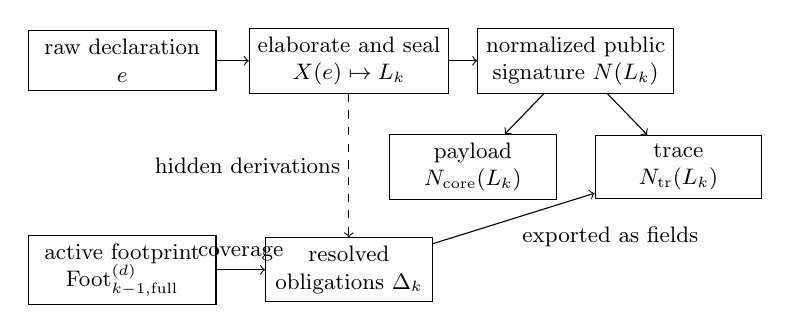
\begin{tikzpicture}[scale=0.9, transform shape,
  every node/.style={font=\small},
  box/.style={draw, align=center, minimum width=2.65cm, minimum height=0.85cm},
  smallbox/.style={draw, align=center, minimum width=2.35cm, minimum height=0.75cm}]
  \node[box] (raw) at (-3.2,1.5) {raw declaration\\$e$};
  \node[box] (seal) at (0,1.5) {elaborate and seal\\$X(e)\mapsto L_k$};
  \node[box] (norm) at (3.2,1.5) {normalized public\\signature $N(L_k)$};
  \node[smallbox] (core) at (1.75,0) {payload\\$N_{\mathrm{core}}(L_k)$};
  \node[smallbox] (trace) at (4.65,0) {trace\\$N_{\mathrm{tr}}(L_k)$};
  \node[box] (foot) at (-3.2,-1.45) {active footprint\\$\Foot_{k-1,\mathrm{full}}^{(d)}$};
  \node[smallbox] (delta) at (0,-1.45) {resolved\\obligations $\Delta_k$};
  \draw[->] (raw) -- (seal);
  \draw[->] (seal) -- (norm);
  \draw[->] (norm) -- (core);
  \draw[->] (norm) -- (trace);
  \draw[->] (foot) -- node[above] {coverage} (delta);
  \draw[->] (delta) -- node[below right] {exported as fields} (trace);
  \draw[->,dashed] (seal) -- node[left] {hidden derivations} (delta);
\end{tikzpicture}
\caption{Sealed-layer export decomposition behind the Integration Trace Principle. The payload part contributes $\kappa_k$ new public schemas. The active footprint generates $\Delta_k$ resolved obligations, and opacity exports their field types as trace schemas while hiding the derivations that inhabit them. Hence $S_{\mathrm{bas}}(L_k)\cong S_{\mathrm{core}}(L_k)\uplus S_{\mathrm{tr}}(L_k)$.}
\label{fig:trace-principle}
\end{figure}

\begin{rem}
\label{rem:trace-native-vs-api}
The trace principle counts kernel-level extensions and promoted interface packages uniformly. In both cases the public export has a payload part and a trace part. The only difference is the kind of primitive datum involved: for native extensions the payload contributes new reduction heads and the trace contributes defining clauses, whereas for promoted packages the payload contributes new exported operators and the trace contributes comparison or transport witnesses.
\end{rem}

\section{Semantic adequacy of the fixed raw extension calculus}
\label{sec:bridge}

The counting calculus of \autoref{sec:framework} is intended to measure explicit extension declarations over the fixed cubical core~$C$, not a freestanding payload calculus detached from syntax. This section spells out the semantic adequacy bridge for the fixed raw extension calculus of \autoref{def:surface-extension}. Raw payload, action, comparison, algebraic-payload, and packaged horn-boundary declarations normalize to sealed public signatures; sealing exports only their opaque public interfaces; and counting is performed on the normalized public signature of that export. The statement is intentionally narrower than an arbitrary Cubical Agda elaboration theorem: Cubical Agda is the mechanization environment, while the theorem target is the raw extension calculus defined here.

\begin{defi}[Semantic structural obligations]
\label{def:semantic-structural-obligations}
A \emph{semantic structural obligation} for a semantic sealed layer
$E_{n+1}$ is an interface field required to interpret the new payload against
the opaque public interfaces already exported by earlier sealed layers. Unary
obligations interpret raw action clauses, binary obligations interpret raw
comparison clauses, and higher horn-shaped obligations interpret raw horn
clauses. This excludes user-authored higher payload constructors: those are
semantic content of $K_{n+1}$, not automatically generated structural trace in
$T_{n+1}$.
\end{defi}

\begin{rem}[Adequacy package and status]
\label{rem:semantic-adequacy-package}
For a general cubical foundation~$F$, the semantic reading of the theorem is
parametric in a raw adequacy package~$A$. The package contains the following
clauses.
\begin{enumerate}
  \item \emph{Raw soundness:} every well-typed raw payload, action,
  comparison, or horn clause has the corresponding semantic interpretation.
  \item \emph{Raw completeness for admissible structural obligations:} every
  admissible semantic structural obligation of the fixed sealing discipline is
  represented by one of the raw clause classes of
  \autoref{def:raw-structural-clauses}.
  \item \emph{Support preservation:} normalization preserves the historical
  support set of every primitive trace field.
  \item \emph{Primitive/derived preservation:} normalization and presentation
  equivalence preserve whether a field is primitive or transparently derived.
  \item \emph{Cardinality preservation:} payload size, trace size, exported
  interface cardinality, and the minimal opaque cost~$\mu$ are preserved by the
  raw-to-normalized-signature bridge.
\end{enumerate}
In this paper these clauses are mechanized for the fixed raw extension calculus
listed in \autoref{rem:bridge-target}; a transfer to an arbitrary Cubical Agda
program or to a different cubical calculus remains conditional on supplying the
corresponding adequacy package. The downstream depth and recurrence statements
therefore use semantic language only through this explicit bridge.
\end{rem}

\subsection{Presentation steps and canonical normal forms}

\begin{defi}[Presentation-step generators]
\label{def:presentation-steps}
Presentation equivalence for admissible declarations is generated by the following local moves on normalized public telescopes:
\[
\begin{array}{ll}
  \mathsf{reassocSigma}              & \text{reassociate or flatten an iterated dependent sum;}\\
  \mathsf{splitRecord}               & \text{split a single-constructor record or shell into its fields;}\\
  \mathsf{bundleRecord}              & \text{rebundle such a field telescope into a record or shell;}\\
  \mathsf{curryPi}                   & \text{turn a product argument into an iterated function telescope;}\\
  \mathsf{uncurryPi}                 & \text{perform the inverse uncurrying step;}\\
  \mathsf{transportField}            & \text{move a field along an already exported equality;}\\
  \mathsf{transparentAliasInsert}    & \text{insert a transparently definable alias field;}\\
  \mathsf{transparentAliasDelete}    & \text{delete such an alias field;}\\
  \mathsf{duplicateDerivedDelete}    & \text{delete a duplicate derived trace field.}
\end{array}
\]
Their reflexive, symmetric, and transitive closure is the relation $e\approx e'$ used in \autoref{def:mu}. The list is also the scope of the raw bridge: it covers the raw constructors of \autoref{def:surface-extension}, namely payload telescopes, action clauses, comparison and transport clauses, algebraic payload packages, export selections, and packaged horn-boundary clauses. It does not include arbitrary source-language rewrites or a parser-level equivalence for Cubical Agda programs.
\end{defi}

\begin{prop}[Counting normalization is stable under presentation steps]
\label{prop:normal-form-stability}
Each generator of \autoref{def:presentation-steps} preserves the canonical counting normal form up to telescope isomorphism, preserves primitive-versus-derived tags, and preserves historical support. Consequently, if $e\approx e'$, then $N(e)\cong N(e')$, $\Prim(N_{\mathrm{tr}}(e))\cong \Prim(N_{\mathrm{tr}}(e'))$, and $\mu(e)=\mu(e')$.
\end{prop}

\begin{proof}
For reassociation, record splitting, rebundling, currying, and uncurrying, both sides elaborate to the same sealed dependent typing judgment with a differently bracketed public telescope; flattening the $\Sigma$-spine and normalizing the $\Pi$-telescope therefore returns the same ordered atomic fields up to canonical renaming. The transport move uses only an equality already exported by an earlier sealed signature, so it changes a field's presentation but not the irreducible prior layers on which the field depends. Transparent alias insertion and deletion add or remove fields whose inhabitants are uniformly synthesized from existing data; such fields are tagged derived and never contribute to the primitive trace count. Duplicate-derived deletion removes only a second copy of an already derived field. Hence every generator preserves the primitive classes and their support. Closure under reflexivity, symmetry, and transitivity gives the result for $e\approx e'$.

In the artifact this is the theorem-facing contract of \AgdaPath{Metatheory/PresentationEquivalence.agda}, \AgdaPath{Metatheory/TraceCostNormalForm.agda}, and \AgdaPath{Metatheory/MuInvariance.agda}: the explicit \AgdaPath{PresentationStep} constructors preserve trace support and primitive cost, and the induced presentation-equivalence relation preserves~$\mu$. The paper does not require a stronger global confluence theorem for arbitrary syntax; it requires uniqueness of the counted normal form for this generated presentation relation, which is exactly the invariant used here.
\end{proof}

\subsection{Elaboration and public signatures}

\begin{thm}[Elaboration soundness for sealed exports]
\label{thm:elaboration}
Every admissible surface extension declaration~$e$ over a state~$\B_n$ determines:
\begin{enumerate}
  \item an elaborated candidate
  \[
    X(e) := (X_{\mathrm{core}}(e), \Gcal_{\mathrm{obl}}(e)),
  \]
  \item a sealed layer $L(e)$ exported through the opaque public interface selected by~$\sigma$,
  \item and a normalized public signature
  \[
    N(e) = N(\mathsf{Elab}(e))
  \]
  obtained from that exported interface by counting normalization.
\end{enumerate}
In particular, the candidate calculus of \autoref{sec:framework} is the image of admissible surface extensions under elaboration and sealing.
\end{thm}

\begin{proof}
By \autoref{def:surface-extension} and \autoref{def:elaboration}, the payload telescope $\Gamma_{\mathrm{new}}$ elaborates to new core declarations, while $\Gamma_{\mathrm{act}}$ and $\Gamma_{\mathrm{cmp}}$ elaborate to the clauses witnessing the required interaction with the active interface of~$\B_n$. Admissibility means precisely that these clauses type-check and discharge the induced coherence obligations, so the result packages into a candidate $X(e)$ together with an opaque exported layer~$L(e)$. Applying the counting normal form of \autoref{def:atomic-schema} to the resulting public telescope yields $N(e)$. Thus every admissible surface extension gives rise canonically to the candidate-and-sealed-layer data used in \autoref{sec:framework}.
\end{proof}

\begin{thm}[Adequacy of normalized public signatures]
\label{thm:adequacy}
\label{thm:semantic-adequacy}
Let $e$ be an admissible surface extension over~$\B_n$ and let $L(e)$ be its sealed export. Then:
\begin{enumerate}
  \item every field of $N(e)$ comes from a field of the sealed public interface of~$L(e)$; counting normalization introduces no new primitive public datum;
  \item every field of $N(e)$ is either a payload schema contributed by $\Gamma_{\mathrm{new}}$ or a trace schema arising from a resolved obligation of~$X(e)$;
  \item every irreducible payload or trace schema visible after sealing occurs as a field of~$N(e)$;
  \item the synthetic quantities $P(X(e))$, $S(L(e))$, $\Delta(X(e)\mid\B_n)$, $\mu(e)$, $\ObSig_k(X(e))$, $\Ix_k(X(e))$, and $\Real_k(X(e))$ are exactly the corresponding payload, public-signature, abstract latency, minimal opaque cost, obligation signature, primitive index set, and realized obligation object computed from~$N(e)$ and its trace part.
\end{enumerate}
\end{thm}

\begin{proof}
Point~(1) is immediate from \autoref{def:elaboration} and \autoref{def:atomic-schema}: the normalization procedure only flattens the exported telescope and discards uniformly synthesized fields, so it cannot create a new primitive field not already present in the sealed typing judgment. Point~(2) is the surface-language form of the decomposition proved abstractly in \autoref{thm:trace}: after elaboration and sealing, every visible field is either newly introduced payload or the public trace of a resolved interaction with prior interface data. Point~(3) follows because counting normalization removes only presentation artifacts: reassociation of telescopes, transparently derivable fields, and other data uniformly synthesized by definitional equality or the generic structure of the ambient cubical calculus. Thus every irreducible field that remains visible after sealing survives into $N(e)$, and no extra irreducible field is created by normalization. Point~(4) is then immediate from the definitions of payload size, public schema set, minimal opaque cost, integration latency, induced obligation signatures, primitive index sets, and realized obligation objects in \autoref{sec:framework} and \autoref{sec:coherence}: those quantities are computed exactly from the normalized public signature and its induced obligations.
\end{proof}

\begin{prop}[Necessity of irreducible public fields]
\label{prop:irreducible-necessary}
Let $e$ be an admissible surface extension over~$\B_n$, and let $\phi$ be an irreducible field of~$N(e)$. If $e' \approx e$, then $N(e')$ contains a canonically corresponding irreducible field~$\phi'$. Equivalently, no presentation-equivalent declaration can delete an irreducible payload or trace schema from the sealed public signature.
\end{prop}

\begin{proof}
By presentation equivalence, $e$ and $e'$ determine the same sealed public typing judgment up to definitional equality, canonical telescope isomorphism, and transparent internal normalization. If the irreducible field~$\phi$ were absent from~$N(e')$, then one of two things would have to happen: either the public typing judgment of~$e'$ would genuinely omit that field, contradicting $e' \approx e$, or the field would have to be uniformly reconstructible from the remaining exported data by those transparent operations. But \autoref{def:atomic-schema} declares $\phi$ irreducible precisely by excluding that second possibility. Hence $\phi$ must survive in every presentation-equivalent normalized public signature.
\end{proof}

\begin{prop}[Canonical normalized presentations]
\label{prop:canonical-presentation}
If $e \approx e'$, then $N(e)$ and $N(e')$ are canonically isomorphic, and their trace parts $N_{\mathrm{tr}}(e)$ and $N_{\mathrm{tr}}(e')$ are canonically isomorphic as well. Consequently every presentation-equivalence class admits a canonical normalized public signature up to isomorphism, and
\[
  \mu(e) = |N_{\mathrm{tr}}(e)|.
\]
\end{prop}

\begin{proof}
Presentation equivalence identifies elaborated sealed extensions whenever they induce the same public typing judgment up to definitional equality, canonical telescope isomorphism, and transparent internal normalization. The counting normal form forgets exactly those presentation differences and nothing more, so $N(e)$ and $N(e')$ are canonically isomorphic. By \autoref{thm:adequacy}, the payload/trace decomposition is part of the sealed typing judgment itself, so the trace subfamilies correspond under that isomorphism. By \autoref{prop:irreducible-necessary}, no presentation-equivalent declaration can remove an irreducible trace field from the normalized public signature unless that field was already transparently reconstructible. Hence every representative of the class has the same canonical irreducible trace cardinality, so the minimum in \autoref{def:mu} is attained by $N_{\mathrm{tr}}(e)$ itself and equals~$|N_{\mathrm{tr}}(e)|$.
\end{proof}

\begin{thm}[Computational replacement on canonical trace presentations]
\label{thm:computational-replacement}
Let $X$ be a candidate over~$\B_n$, let $k$ be a history depth, and let $S$ be the canonical normalized trace signature attached to the depth-$k$ trace family of~$X$. Let $P$ and $Q$ be two presented trace telescopes whose counting normal forms are~$S$, and let $\phi$ be a presented trace field of~$P$. Suppose there is a lower-arity boundary subfamily $\partial_\phi$ and a cubically synthesized term
\[
  t_\phi(\partial_\phi),
\]
built only from $\hcomp$, $\transp$, $\mathsf{hfill}$, definitional equality, and the transparent structural operations already quotiented by counting normalization, such that after passage to~$S$ the field corresponding to~$\phi$ is judgmentally reconstructed from lower-arity boundary data and is therefore tagged as transparently derived rather than primitive. Then:
\begin{enumerate}
  \item $P$ and~$Q$ are presentation-equivalent representations of the same canonical trace signature;
  \item in the $\mu$-minimal part of the canonical normalized trace signature represented by~$S$, the field corresponding to~$\phi$ is absent as an irreducible primitive trace field;
  \item every other irreducible primitive trace field of~$P$ corresponds canonically to one of~$Q$.
\end{enumerate}
\end{thm}

\begin{proof}
Because both~$P$ and~$Q$ normalize to the same canonical trace signature~$S$, they are presentation-equivalent representations of one canonical public trace interface. The derivedness of~$\phi$ is not being assumed from the conclusion: it is witnessed by the displayed transparent term $t_\phi(\partial_\phi)$ in the fixed derivability relation generated by cubical Kan operations and the presentation steps of \autoref{def:presentation-steps}. Thus the normalized image of~$\phi$ is reconstructed from lower-arity boundary data, so its canonical primitive-cost tag is \emph{transparently derived} rather than \emph{requires primitive}. Therefore~$\phi$ is excluded from the $\mu$-minimal part of~$S$, which retains only irreducible primitive trace fields. Since primitive-cost tags are preserved under passage between presentations of the same canonical signature, every other irreducible primitive field of~$P$ corresponds canonically to one of~$Q$. Thus the replacement step changes only the presentation of the trace telescope, not the canonical primitive content measured by~$\mu$.
\end{proof}

\begin{rem}[Exact scope of the mechanized fixed raw bridge]
\label{rem:bridge-target}
The formal bridge in the accompanying Agda development is a three-part package for the fixed raw extension calculus, not an additional cubical metatheory and not a parser for arbitrary Cubical Agda source:
\begin{enumerate}
  \item raw admissible surface declarations are connected, via elaboration and sealing, to canonical normalized signatures by \AgdaPath{Metatheory/RawStructuralSyntax.agda}, \AgdaPath{Metatheory/RawStructuralTyping.agda}, and \AgdaPath{Metatheory/SurfaceNormalizationBridge.agda};
  \item presentation-equivalent canonical trace normal forms preserve support, primitive cost, and~$\mu$ by the explicit \AgdaPath{PresentationStep} generators in \AgdaPath{Metatheory/PresentationEquivalence.agda} and \AgdaPath{Metatheory/MuInvariance.agda};
  \item the resulting canonical normalized signatures are matched with the counted-interface quantities by \AgdaPath{normalized-signature-matches-counted-interface}, and well-typed raw structural clauses are identified with the horn-generated trace image by \AgdaPath{Metatheory/SurfaceToHornImage.agda}.
\end{enumerate}
In particular, \autoref{thm:computational-replacement} itself remains formalized on canonical trace presentations, while the bridge modules connect admissible raw declarations to that interface and to the counted abstract interface. What is deliberately outside the theorem is a general parser or elaboration theorem for the whole Cubical Agda language.
\end{rem}

\begin{cor}[Minimal opaque cost agrees with abstract coherence cost]
\label{cor:mu-delta}
For every admissible surface extension declaration~$e$ over~$\B_n$,
\[
  \mu(e) = |\Prim(N_{\mathrm{tr}}(e))| = \Delta(X(e)\mid\B_n).
\]
If $e_k$ is the declaration whose sealing exports~$L_k$, if $\mu_k := \mu(e_k)$,
and if $S_{\mathrm{bas}}(L_k)$ is any basis family of~$L_k$, then
\[
  |S_{\mathrm{bas}}(L_k)| = \kappa_k + \mu_k.
\]
\end{cor}

\begin{proof}
By \autoref{thm:adequacy}, the trace part of $N(e)$ records exactly the
irreducible public trace schemas arising from resolved obligations of~$X(e)$.
By \autoref{prop:canonical-presentation}, $\mu(e)$ is exactly the cardinality
of the primitive part of that canonical trace signature. By \autoref{thm:canonicity}, there is one and
only one irreducible primitive trace schema for each basis site of the active
interface, so that cardinality is precisely $\Delta(X(e)\mid\B_n)$. The final
formula is then the trace-principle decomposition of \autoref{thm:trace},
rewritten using $\mu_k=\Delta(X(e_k)\mid\B_{k-1})$; its right-hand side is
well defined for any basis family by \autoref{thm:basis-choice}.
\end{proof}

\begin{lem}[Trace-cost dictionary]
\label{lem:trace-cost-dictionary}
Let $e_k$ be an admissible fully coupled declaration whose sealing exports
$L_k$. Then the following quantities are the same cardinality, read at their
respective levels:
\[
  \mu(e_k)
  =
  |\Prim(N_{\mathrm{tr}}(e_k))|
  =
  \Delta(X(e_k)\mid\B_{k-1})
  =
  |S_{\mathrm{tr}}(L_k)|.
\]
Moreover the primitive basis of the exported layer decomposes as
\[
  |S_{\mathrm{bas}}(L_k)|
  =
  |S_{\mathrm{core}}(L_k)|+|S_{\mathrm{tr}}(L_k)|
  =
  \kappa_k+\mu_k.
\]
Thus the recurrence later uses a cardinality identity obtained from normalized
public signatures, not an additional semantic growth assumption.
\end{lem}

\begin{proof}
The first equality is the definition of minimal opaque cost on the canonical
trace presentation, the second is \autoref{cor:mu-delta}, and the third is the
trace part of the sealed export decomposition in \autoref{thm:trace}. The
second displayed formula is the primitive-class restriction of the same
payload/trace decomposition, with $|S_{\mathrm{core}}(L_k)|=\kappa_k$ by
\autoref{def:payload}. Invariance under presentation replacement follows from
\autoref{lem:basis-invariants}.
\end{proof}

\begin{defi}[Factorization-complete public trace export]
\label{def:factorization-complete}
Let $L_k$ be a sealed layer with $k \geq 2$. We say that its public trace
export is \emph{factorization-complete} if, after choosing any admissible
surface declaration whose sealing exports~$L_k$ and reading its canonical
normalized trace signature, the following data are available for the next
remote-comparison step:
\begin{enumerate}
  \item the adjacent unary bridge from $L_k$ to~$L_{k-1}$;
  \item the binary comparison trace witnessing the composite comparison from
  $L_k$ to~$L_{k-2}$ through~$L_{k-1}$;
  \item the degenerate or structural faces needed to assemble the corresponding
  open $3$-box, generated transparently by definitional equality, transport
  along already exported equalities, and the generic structural operations
  already quotiented by counting normalization.
\end{enumerate}
Equivalently, the next horn-extension problem involving~$L_k$ can be posed
using only exported public trace fields and transparent structural operations,
without reopening the hidden derivation that discharged the original sealing
obligations.
\end{defi}

\begin{thm}[Sealed layers export factorization-complete trace data]
\label{thm:factorization-complete}
Every sealed layer $L_k$ with $k \geq 2$ in the fixed fully coupled cubical
extension calculus has factorization-complete public trace export.
\end{thm}

\begin{proof}
Choose an admissible surface declaration~$e_k$ whose sealing exports~$L_k$.
By \autoref{thm:trace}, the public export of~$L_k$ decomposes into new payload
and trace, and by \autoref{thm:adequacy} every irreducible trace schema visible
after sealing appears in the canonical normalized trace signature
$N_{\mathrm{tr}}(e_k)$. Because $L_k$ was sealed as a globally acting layer
against the active interface, its resolved trace obligations include the
adjacent action on~$L_{k-1}$ and the binary comparison against the already
exported comparison between $L_{k-1}$ and~$L_{k-2}$. Hence the corresponding
unary bridge and binary comparison trace occur as public fields of
$N_{\mathrm{tr}}(e_k)$.

The remaining faces needed for the next open $3$-box are not extra primitive
obligations. They are degenerate composites, reindexings, and transports along
already exported equalities, so they are generated transparently by the
structural operations already quotiented in counting normalization. By
\autoref{prop:irreducible-necessary} and
\autoref{prop:canonical-presentation}, passing to a presentation-equivalent
declaration cannot delete the irreducible unary or binary trace fields just
identified; it can only rewrite them into canonically isomorphic normalized
form. Therefore the factorization data are exported stably at the level of
canonical normalized public signatures and can be reused without reopening the
hidden sealing derivation. This is exactly factorization completeness.
\end{proof}

\begin{rem}[Use of the bridge in later sections]
\label{rem:bridge-to-counting}
The results of \autoref{sec:coherence} and \autoref{sec:mechanization} invoke surface syntax only through \autoref{rem:bridge-target}. Once an admissible declaration has been identified with its canonical normalized signature and the corresponding counted-interface data, the later depth, factorization, and recurrence theorems are applications of the abstract candidate-and-obligation calculus.
\end{rem}

\section{Normal forms for structural trace}
\label{sec:trace-normal-forms}

The adequacy bridge reduces the paper-facing semantic question to a small
normal-form question about the trace part of a sealed public signature. After
normalization, every admissible structural trace field is read in one of three
roles: unary action trace, binary comparison trace, or a higher horn package.
The roles are semantic roles, not merely syntactic tags. Each carries explicit
historical support data, and each role determines whether the field is a
candidate primitive public trace field or a derived one.

\begin{table}[t]
\centering
\caption{Normal forms for structural trace.}
\label{tab:trace-normal-forms}
\small
\begin{tabular}{@{}p{0.22\linewidth}p{0.28\linewidth}p{0.23\linewidth}p{0.17\linewidth}@{}}
\toprule
Normal role & Semantic content & Historical support & Primitive status \\
\midrule
Unary action trace & Action of the new payload on one exported interface site & one prior public field & primitive candidate unless transparently generated \\
Binary comparison trace & Compatibility between two already exported actions, transports, or comparison witnesses & two prior public fields, or adjacent composite trace through them & primitive candidate; necessary in general by the swap obstruction \\
Higher horn package & Boundary plus missing face/filler data for a higher structural obligation & a horn boundary assembled from unary and binary public trace & derived when the boundary is filled by $\hcomp$, $\transp$, and $\mathsf{hfill}$ \\
\bottomrule
\end{tabular}
\end{table}

Unary action trace is the image of a raw action clause. It records how the new
sealed payload acts on one previously exported basis site. Binary comparison
trace is the image of raw comparison or transport clauses. It records that two
publicly visible routes, already determined by action data and prior trace,
agree in the way required for later sealed extensions to use them opaquely.
These two roles are the only roles that may contribute irreducible primitive
public trace fields in a $\mu$-minimal normalized signature.

The higher role is different. A horn package may still appear in the exact
realized obligation object, but its public trace field is primitive only if the
fixed cubical structure cannot compute it from its displayed boundary. In the
cubical setting of this paper, the derivedness witness is the actual boundary
computation: $\hcomp$ synthesizes the missing face, $\transp$ aligns it along
the exported comparison data, and $\mathsf{hfill}$ packages the filler. Thus
the higher field is not declared derived by convention; it is derived because a
term built from the semantic Kan operations reconstructs it from lower-arity
public boundary trace. This is the normal-form content used by
\autoref{thm:computational-replacement}, \autoref{lem:horn-reduction}, and
\autoref{thm:higher-elim}.

The same normal form also separates structural trace from payload. A
user-supplied higher algebraic operation, higher HIT constructor, or other
primitive higher-dimensional datum is part of the payload telescope~$K_n$ when
it is authored as new semantic content. It is not reclassified as structural
trace merely because it has higher arity or dimension. It becomes a structural
horn package only when it is a sealing obligation whose boundary is built from
previous public interface data and whose role is to integrate the new payload
with that interface.

\section{Obligation Depth, Minimal-Signature Depth, and the Dichotomy}
\label{sec:coherence}

\subsection{Induced obligations and historical arity}

\begin{defi}[Induced obligation signatures and realized objects]
\label{def:obligations}
For a candidate~$X$ sealed against a historical interface of depth~$k$, we distinguish five objects.
\[
\begin{array}{rcl}
  \ObSig_k(X) &:& \text{the finite normalized obligation signature},\\
  \Ix_k(X) &:& \text{the finite set of primitive schema indices in } \ObSig_k(X),\\
  \Real_k(X) &:& \text{the dependent type or space interpreting } \ObSig_k(X),\\
  \Prim_k(X) &:& \text{the primitive irreducible sub-signature},\\
  \Der_k(X) &:& \text{the derived or transparently synthesized sub-signature}.
\end{array}
\]
The signature $\ObSig_k(X)$ is read in the counting normal form of \autoref{def:atomic-schema}: we quotient by canonical telescope isomorphisms and tag each field as primitive or derived. The set $\Ix_k(X)$ indexes only primitive fields, while $\Real_k(X)$ is the actual dependent object whose inhabitants discharge the exact obligations. Thus stabilization and contractibility theorems below are statements about $\Real_k(X)$, whereas minimal public cost and arity elimination are statements about $\Prim_k(X)$ and the trace part of normalized public signatures.

When a potential higher-dimensional coherence problem appears with one face left free, the corresponding exact obligation object is represented in $\Real_k(X)$ by the horn-extension type of the missing face together with a filler, rather than by the type of fillers for a completely fixed boundary. Since the interface grows cumulatively, the primitive index sets and realized objects are related by restriction maps
\[
  \Ix_1(X) \to \Ix_2(X) \to \Ix_3(X) \to \cdots,
  \qquad
  \Real_1(X) \to \Real_2(X) \to \Real_3(X) \to \cdots,
\]
with the direction of comparison determined by exposing more historical interface.
\end{defi}

\begin{rem}
\label{rem:present-vs-cost}
The paper uses the following five-way taxonomy.
\begin{center}
\small
\begin{tabular}{@{}p{0.31\linewidth}p{0.61\linewidth}@{}}
\toprule
Status & Meaning \\
\midrule
Present obligation type & A normalized obligation type genuinely appears in some $\Real_k(X)$ and therefore belongs to the exact metatheoretic stabilization problem. \\
Contractible obligation type & The obligation type is still present in $\Real_k(X)$, but its fiber is canonically contractible; this is not yet a statement about minimal public syntax. \\
Transparently derived field & A field is part of the sealed typing judgment but is uniformly reconstructible from other exported data by definitional equality, transport, or the generic structural operations already quotiented by counting normalization. \\
Eliminated from a $\mu$-minimal signature & A primitive field may occur in some presentation, but every canonical $\mu$-minimal normalized public signature removes it after passage through the explicit presentation-equivalence generators and the fixed raw bridge of \autoref{rem:bridge-target}. \\
Absent from the exact obligation object & No normalized obligation type of that kind occurs in the relevant $\Real_k(X)$. \\
\bottomrule
\end{tabular}
\end{center}
Obligation depth~$d_{\mathrm{obl}}$ is a statement about exact normalized obligation types as realized in $\Real_k(X)$. Minimal-signature depth~$d_\mu$ asks a different question, namely which primitive trace fields survive in canonical normalized public form. A bound on~$d_\mu$ therefore does not by itself produce a chronological window. Accordingly, ``contractible'', ``transparently derived'', ``eliminated from a minimal presentation'', and ``absent'' are never used interchangeably in this paper. The schematic separation in \autoref{rem:toy-separation} below is the motivating toy case: a depth-three horn factor remains present in the exact realized obligation object, is contractible as a type, and contributes no irreducible primitive field to~$\mu$.
\end{rem}

\begin{defi}[Historical support and arity]
\label{def:arity}
For a normalized obligation~$o$, let $\Supp(o)$ be the set of sealed layers whose atomic exported schemas occur irreducibly in the counting normal form of the typing derivation of~$o$ after each prior layer has been collapsed to its opaque interface. Its \emph{historical arity} is
\[
  a(o) := |\Supp(o)|.
\]
\end{defi}

\begin{rem}
\label{rem:deep-lookups}
Historical arity counts independent prior layers, not textual age. A direct lookup to an old exported theorem is still unary, because it lands in one opaque interface. Multi-layer debt arises only when the new layer must cohere simultaneously with several independent prior exports.
\end{rem}

\begin{lem}[Arity-to-dimension correspondence]
\label{lem:arity-dimension}
An irreducible obligation of historical arity~$k$ requires a $k$-dimensional coherence cell. Arity~$1$ produces substitution or transport data, arity~$2$ produces a naturality square or homotopy, and arity $k \geq 3$ would require a genuine higher filler.
\end{lem}

\begin{proof}
The statement is a dimension assignment for the structural-integration grammar of \autoref{def:surface-extension}. Unary action clauses in $\Gamma_{\mathrm{act}}$ mention one prior opaque signature, so their normalized obligation is a single transport or comparison path. Binary comparison clauses in $\Gamma_{\mathrm{cmp}}$ mention two independent prior signatures and compare the two unary composites through them, hence form a square or homotopy. The horn-boundary clauses are generated inductively: passing from arity $k-1$ to arity~$k$ adjoins one further remote layer to an already normalized boundary and asks for the missing comparison face plus a filler of the resulting open box. Therefore the marginal arity-$k$ structural obligation is a $k$-dimensional horn-extension cell. Since support is computed after opacity and counting normalization, transparent aliases, record rebundlings, and transports along already exported equalities cannot increase this dimension assignment.
\end{proof}

\subsection{Definition of obligation depth and minimal-signature depth}

\begin{defi}[Obligation depth and minimal-signature depth]
\label{def:depth}
A foundation, equivalently a fixed extension calculus together with its sealing discipline, has \emph{obligation depth}~$d_{\mathrm{obl}}$ if $d_{\mathrm{obl}}$ is the least integer such that for every candidate~$X$ and all $k \geq d_{\mathrm{obl}}$ there is a canonical equivalence
\[
  \Real_k(X) \simeq \Real_{d_{\mathrm{obl}}}(X).
\]
It has \emph{minimal-signature depth}~$d_\mu$ if $d_\mu$ is the least integer such that every admissible surface extension declaration~$e$ is presentation-equivalent to a declaration~$e'$ whose primitive trace sub-signature $\Prim(N_{\mathrm{tr}}(e'))$ contains no irreducible primitive historical field of arity greater than~$d_\mu$.

When the paper says simply ``coherence depth,'' it means obligation depth, not yet a chronological-window theorem.
\end{defi}

\begin{defi}[Chronological window size]
\label{def:chronological-window}
A foundation has \emph{chronological window size} at most~$d$ if every admissible sealing step at stage~$n+1$ has the following property after passage to the canonical normalized public signature: each surviving primitive trace field has support contained in
\[
  \{L_n,L_{n-1},\dots,L_{n-d+1}\},
\]
and every comparison with a remote layer $L_{n-r}$ for $r\geq d$ is presentation-equivalent to a trace term factored through the exported normalized signatures of those $d$ recent layers. Equivalently, remote history may still occur in exact derived horn factors, but it contributes no primitive public trace field outside the recent window.
\end{defi}

The point of \autoref{def:depth} is that beyond depth~$d_{\mathrm{obl}}$, the realized obligation objects themselves stop changing up to canonical equivalence. This is stronger than saying merely that deeper history contributes no new minimal opaque cost or that $d_\mu$ is bounded. Once that exact stabilization has been upgraded to a genuine chronological window, the size of the primitive active basis interface controls the recurrence law for integration debt.

\begin{rem}
\label{rem:arity-vs-chronology}
\autoref{def:depth} records two depth notions. The obligation-depth bound~$d_{\mathrm{obl}}$ is a stabilization statement about \emph{realized obligation objects}; the minimal-signature bound~$d_\mu$ is a statement about canonical normalized public signatures. Neither should be read as saying that a bound on coherence dimension automatically identifies the chronological layers that must still be inspected primitively. In particular, an arity-two obligation could in principle couple a new layer to a remote historical layer. To extract a genuine time window from a dimensional bound one needs an additional factorization theorem showing that such remote binary comparisons are already generated by recently exported traces. In the cubical univalent case, this passage from arity to chronology is supplied by \autoref{lem:telescopic}.
\end{rem}

\begin{rem}[Equality conventions]
\label{rem:equality-conventions}
The symbols in this section live at different levels. The equivalence $\Real_k(X)\simeq\Real_j(X)$ is an equivalence of realized dependent obligation objects. The isomorphism $N(e)\cong N(e')$ is a canonical telescope isomorphism of normalized public signatures. A field being \emph{definitionally equal} to a synthesized trace term means equality after elaboration and counting normalization in the fixed presentation relation of \autoref{def:presentation-steps}. Path equalities such as the swap obstruction are internal cubical paths. Finally, ``eliminated from a $\mu$-minimal signature'' is a quotient-level statement: the field may occur in a presentation, but not as a primitive field in the canonical normalized trace class measured by~$\mu$.
\end{rem}

\begin{rem}[Statement-level audit]
\label{rem:statement-level-audit}
The numbered results in the paper are intentionally sorted by level. The table
below records the intended reading so that later uses do not move silently
between syntax, realized types, primitive signatures, chronology, and
cardinality.
\begin{center}
\small
\begin{tabular}{@{}p{0.28\linewidth}p{0.22\linewidth}p{0.42\linewidth}@{}}
\toprule
Results & Level & What is asserted \\
\midrule
\autoref{thm:basis-choice}, \autoref{lem:basis-invariants},
\autoref{prop:normal-form-stability}, \autoref{prop:canonical-presentation}
& normalized syntax & Primitive class sets, basis transversals, supports, and
canonical presentations are invariant under presentation equivalence. \\
\autoref{thm:coverage}, \autoref{prop:basis-minimality},
\autoref{thm:canonicity}
& admissibility and cardinality & Full coupling forces exactly one primitive
trace schema per active basis site under the bundled counting convention. \\
\autoref{thm:trace}, \autoref{cor:mu-delta},
\autoref{lem:trace-cost-dictionary}
& signature decomposition and cardinality & Sealed exports split into payload
and trace parts, and $\mu$ is identified with the primitive trace cardinality. \\
\autoref{lem:arity-dimension}, \autoref{thm:extensional},
\autoref{thm:upper}, \autoref{cor:contractible-factor},
\autoref{thm:horn-interface}, \autoref{cor:cubical-horn-interface}
& realized objects & Exact stabilization and contractible-factor claims are
equivalences or contractibility statements about $\Real_k(X)$. \\
\autoref{thm:computational-replacement}, \autoref{thm:higher-elim},
\autoref{cor:dmu2}
& primitive public signatures & Higher presented trace fields become derived
in canonical $\mu$-minimal trace signatures; they are not claimed absent from
$\Real_k(X)$. \\
\autoref{thm:factorization-complete}, \autoref{lem:telescopic},
\autoref{cor:chrono-window}
& chronology & Surviving primitive binary support factors through recently
exported normalized signatures. \\
\autoref{thm:adjunction}, \autoref{thm:clutching}, \autoref{cor:d2}
& lower bound and exact depth & Binary sealing data are necessary in the
univalent cubical setting, while higher exact factors stabilize. \\
\autoref{thm:recurrence}, \autoref{cor:depth-two-window-recurrence},
\autoref{cor:d1}, \autoref{cor:fibonacci}, \autoref{cor:phi}
& arithmetic cardinality & Once a chronological window and full footprint are
fixed, the recurrence is a counting theorem for $\mu$ and $\kappa$. \\
\bottomrule
\end{tabular}
\end{center}
\end{rem}

\subsection{\texorpdfstring{Theorem A: extensional systems collapse to $d_{\mathrm{obl}}=1$}{Theorem A: extensional systems collapse to d obl = 1}}

\begin{thm}
\label{thm:extensional}
In Martin-L\"of type theory with UIP, the obligation depth is~$1$.
\end{thm}

\begin{proof}
Under UIP, any two proofs of identity between fixed endpoints are equal. Hence every identity type is a set, and every higher identity type is a proposition; once inhabited, it is contractible. Consider any normalized coherence obligation of dimension at least~$2$. By \autoref{lem:arity-dimension}, it corresponds to a higher identity witness. But in the presence of UIP such a witness is uniquely determined by its boundary and therefore carries no independent data. Thus every obligation of arity at least~$2$ collapses to data already fixed by its unary boundary. Equivalently,
\[
  \Real_k(X) \simeq \Real_1(X)
  \qquad
  (k \geq 1).
\]
Since depth~$0$ would mean the absence of any interaction with the current interface, which is impossible for a nontrivial sealing step, the least stabilizing obligation depth is~$1$.
\end{proof}

\subsection{\texorpdfstring{Theorem B: the fixed cubical calculus has $d_{\mathrm{obl}}=2$}{Theorem B: the fixed cubical calculus has d obl = 2}}

From now on we specialize the paper's fixed theorem object to the fully coupled cubical extension calculus built over the chosen CCHM-style core~\cite{cubical,cchm-hits}, with univalence and Kan composition available in the ambient operational semantics. The next ingredients are deliberately complementary: an exact stabilization theorem for realized obligation objects gives the bound $d_{\mathrm{obl}} \leq 2$; \autoref{thm:higher-elim} gives the separate syntactic bound $d_\mu \leq 2$ on $\mu$-minimal public presentations; recent-history factorization turns the exact depth bound into a genuine two-step time window; and the explicit swap obstruction together with the clutching family give lower-bound witnesses. Together they determine exact obligation depth~$2$.

Univalence and cubical computation play different roles in that argument. Univalence supplies the lower-bound source of genuine binary coherence, witnessed below by the swap obstruction and the clutching family. It does not by itself remove primitive arity-$3$ trace fields or produce exact stabilization of realized obligation objects. Those exact-stabilization and elimination statements use the separate cubical horn-computation package together with recent-history factorization.

One semantic clarification is important before the cubical argument begins. In univalent foundations, types behave as weak $\omega$-groupoids, so the geometric space of fillers for a fixed higher boundary is not generally contractible. The paper therefore does not model a depth-three obligation as the space of fillers for a closed $3$-sphere. After the normalization of \autoref{def:obligations}, the marginal higher-dimensional datum appears instead as a horn-extension problem: an open box with one remote face still free.

It is equally important to delimit the class of obligations under discussion. The paper does not claim that arbitrary internal higher-algebraic structure carried by a candidate disappears from cubical type theory. What is measured here is only \emph{structural integration coherence}: the obligations induced by sealing a globally acting foundational candidate against prior opaque layers. Those obligations arise from the chronological dependency graph of exported payload and trace data, not from arbitrary user-specified higher operations internal to the candidate.

\begin{defi}[Structural horn-extension package]
\label{def:horn-extension-package}
Let $X$ be sealed at stage~$n+1$ and let $k\geq3$. The \emph{remote layer} exposed by the depth-$k$ step is
\[
  R_k(n) := L_{n-k+1}.
\]
For a boundary $\partial:\Real_{k-1}(X)$, the \emph{visible boundary object}
\[
  \partial^{(k)}_{\mathrm{vis}}(X,R_k(n))
\]
consists of the already exported unary traces of $X$ against the recent layers, the binary comparison traces exported by the intervening layers, and all degenerate or transport faces generated transparently from those public traces. The only face not part of this visible boundary is the direct remote comparison between the action of $X$ and the newly exposed layer~$R_k(n)$.

The \emph{missing-data package} is the telescope
\[
  \Gamma^{(k)}_{\mathrm{miss}}(\partial)
\]
of such direct remote comparison faces compatible with the endpoints of $\partial^{(k)}_{\mathrm{vis}}$. For $\gamma:\Gamma^{(k)}_{\mathrm{miss}}(\partial)$, the \emph{filler predicate}
\[
  \mathsf{Fill}^{(k)}_{\partial}(\gamma)
\]
is the type of cubical fillers completing the open $k$-box whose visible faces are $\partial^{(k)}_{\mathrm{vis}}$ and whose missing face is~$\gamma$. The \emph{horn-extension object} is
\[
  H_k(\partial)
  :=
  \sum_{\gamma : \Gamma^{(k)}_{\mathrm{miss}}(\partial)}
  \mathsf{Fill}^{(k)}_{\partial}(\gamma).
\]
This is a horn-extension type, not a closed-filler type. In cubical type theory, the operational semantics provide generic Kan operations such as $\hcomp$, $\compop$, and $\transp$ that solve such horn-extension problems uniformly. The sharp question for this paper is therefore syntactic: does a field of that shape survive as an irreducible trace field in a $\mu$-minimal normalized public signature, or can it be replaced definitionally by a term synthesized from lower-arity boundary data?
\end{defi}

\begin{figure}[t]
\centering
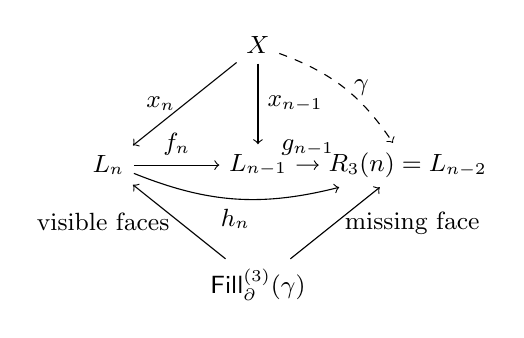
\begin{tikzpicture}[scale=0.95, every node/.style={font=\small}]
  \node (X)  at (0,2.4) {$X$};
  \node (Ln) at (-2,0.8) {$L_n$};
  \node (Lm) at (0,0.8) {$L_{n-1}$};
  \node (Lr) at (2,0.8) {$R_3(n)=L_{n-2}$};
  \node (F)  at (0,-0.8) {$\mathsf{Fill}^{(3)}_{\partial}(\gamma)$};
  \draw[->] (X) -- node[left] {$x_n$} (Ln);
  \draw[->] (X) -- node[right] {$x_{n-1}$} (Lm);
  \draw[->] (Ln) -- node[above] {$f_n$} (Lm);
  \draw[->] (Lm) -- node[above] {$g_{n-1}$} (Lr);
  \draw[->] (Ln) to[bend right=18] node[below] {$h_n$} (Lr);
  \draw[->,dashed] (X) to[bend left=18] node[right] {$\gamma$} (Lr);
  \draw[->] (F) -- node[left] {visible faces} (Ln);
  \draw[->] (F) -- node[right] {missing face} (Lr);
\end{tikzpicture}
\caption{A labeled depth-three horn-extension step. The solid arrows are visible public traces: unary bridges and binary comparison traces already exported by recent sealed layers. The dashed arrow is the missing remote face~$\gamma$ comparing the two composites from $X$ to $L_{n-2}$. The filler predicate asks for the cubical cell completing this open box.}
\label{fig:depth-three-horn}
\end{figure}

\begin{lem}[Syntactic horn reduction for structural integration coherence]
\label{lem:horn-reduction}
\label{thm:semantic-horn-reduction}
Let $X$ be a foundational core candidate sealed at stage~$n+1$ in the fixed fully coupled cubical extension calculus. For every $k \geq 3$ and every boundary $\partial : \Real_{k-1}(X)$, the additional data exposed by adjoining the remote layer $L_{n-k+1}$ are canonically represented by a horn-extension fiber
\[
  H_k(\partial)
  :=
  \sum_{\gamma : \Gamma^{(k)}_{\mathrm{miss}}(\partial)}
  \mathsf{Fill}^{(k)}_{\partial}(\gamma).
\]
Here $\gamma$ is the new remote comparison face between $X$ and $L_{n-k+1}$, while every other face of the box is already exported by the unary and binary traces of the intervening sealed layers as in \autoref{def:horn-extension-package}.
\end{lem}

\begin{proof}
By construction, $\Real_k(X)$ records only structural integration obligations induced by sealing $X$ against opaque prior layers. Earlier layers therefore contribute only their exported payload and trace schemas; arbitrary higher-algebraic structure internal to those layers is invisible at sealing time. Passing from depth $k-1$ to depth~$k$ exposes exactly one additional remote layer, namely $R_k(n)=L_{n-k+1}$. By \autoref{thm:canonicity}, the global action of $X$ contributes exactly one interaction site for each newly exposed primitive generator. Meanwhile, because the intermediate layers were already sealed, their public exports contain the unary bridges and binary comparison traces linking that remote layer to the more recent history; by \autoref{thm:factorization-complete}, the degenerate composition and transport faces needed to assemble the open box are generated transparently from those same exports. Thus the visible boundary is exactly $\partial^{(k)}_{\mathrm{vis}}(X,R_k(n))$ of \autoref{def:horn-extension-package}.

After counting normalization, all faces of the resulting comparison box are fixed except the direct remote comparison face comparing the action of $X$ with the newly exposed remote layer. The possible choices of that face form $\Gamma^{(k)}_{\mathrm{miss}}(\partial)$, and once such a face~$\gamma$ has been chosen the remaining exact obligation is precisely the filler predicate $\mathsf{Fill}^{(k)}_{\partial}(\gamma)$. Therefore the marginal depth-$k$ data are the displayed dependent sum. The depth-three instance is pictured in \autoref{fig:depth-three-horn}; the general case is the same one-step extension of the already normalized boundary by one remote layer.
\end{proof}

\paragraph{A concrete cubical sketch.}
The abstract distinction between payload and trace can be made visible in a small cubical example. Suppose an older sealed layer exports a small Tarski universe with function codes and their decoding equation. A new cohesive layer contributes a genuinely new modal payload \texttt{Flat} together with its unit \texttt{eta}. Everything else needed to make that modality act on the older universe is integration trace: a lifted action on old codes, a comparison between decoding before or after lifting, and the distribution law over old function codes. In the snippet below, the witness \texttt{remote-face} is the point of the example. It is not additional payload. It is exactly the missing comparison face of the open $3$-box determined by the old decoding law together with the new unary and binary trace data, and cubical composition computes it uniformly.

\begin{quote}
\begin{verbatim}
-- Schematic Cubical Agda: old universe + new payload + induced trace

record OldU : Set1 where
  field
    U      : Set
    El     : U -> Set
    Arr    : U -> U -> U
    El-Arr : (A B : U) ->
      Path Set (El (Arr A B)) (El A -> El B)

record Payload : Set1 where
  field
    Flat : Set -> Set
    eta  : {A : Set} -> A -> Flat A

record Trace (L : OldU) (P : Payload) : Set1 where
  open OldU L
  open Payload P
  field
    FlatU         : U -> U
    flat-El       : (A : U) ->
      Path Set (El (FlatU A)) (Flat (El A))
    flat-code-Arr : (A B : U) ->
      Path U (FlatU (Arr A B)) (Arr (FlatU A) (FlatU B))
    flat-Arr      : (A B : U) ->
      Path Set (Flat (El A -> El B))
               (Flat (El A) -> Flat (El B))

module _ (L : OldU) (P : Payload) (T : Trace L P) where
  open OldU L
  open Payload P
  open Trace T

  -- left route:
  --   El (FlatU (Arr A B))
  --     -> Flat (El (Arr A B))
  --     -> Flat (El A -> El B)
  --     -> Flat (El A) -> Flat (El B)

  -- right route:
  --   El (FlatU (Arr A B))
  --     -> El (Arr (FlatU A) (FlatU B))
  --     -> El (FlatU A) -> El (FlatU B)
  --     -> Flat (El A) -> Flat (El B)

  postulate
    left-route  :
      (A B : U) ->
      Path Set (El (FlatU (Arr A B))) (Flat (El A) -> Flat (El B))
    right-route :
      (A B : U) ->
      Path Set (El (FlatU (Arr A B))) (Flat (El A) -> Flat (El B))

  -- The open 3-box says these two boundary composites agree.
  -- This face is transparently derived trace, not new payload.
  remote-face :
    (A B : U) ->
    Path (Path Set (El (FlatU (Arr A B)))
                   (Flat (El A) -> Flat (El B)))
         (left-route A B) (right-route A B)
  remote-face A B = hcomp ...
\end{verbatim}
\end{quote}

Read top-to-bottom, \texttt{Payload} is the human-authored new content, while \texttt{Trace} is the compatibility debt forced by sealing against the old universe. The two routes are the two composites from \texttt{El (FlatU (Arr A B))} to \texttt{Flat (El A) -> Flat (El B)}. The marginal depth-$3$ obligation is not the space of fillers for a closed boundary. It is the horn-extension type whose free component is the remote comparison between those composites and whose second component is the $3$-cell certifying compatibility with the displayed boundary. In a cubical presentation this total extension type is canonically contractible: \texttt{hcomp} computes the missing face and \texttt{hfill} packages the accompanying filler. The extra factor is therefore present but contractible, rather than absent.

\begin{rem}[Toy separation of \texorpdfstring{$d_{\mathrm{obl}}$ and $d_\mu$}{d obl and d mu}]
\label{rem:toy-separation}
The cubical sketch above isolates the separation direction relevant for this paper. Fix $A,B:U$ and let $\partial(A,B)$ be the lower-arity boundary built from \texttt{flat-El}, \texttt{flat-code-Arr}, and \texttt{flat-Arr}. The exact depth-$3$ obligation over that boundary is
\[
  H_3(\partial(A,B))
  :=
  \sum_{\rho : \Gamma^{(3)}_{\mathrm{miss}}(\partial(A,B))}
  \mathsf{Fill}^{(3)}_{\partial(A,B)}(\rho),
\]
whose first component is the would-be remote comparison field \texttt{remote-face}. Cubical composition makes $H_3(\partial(A,B))$ canonically contractible, so this higher obligation is still present in $\Real_3(X)$ even though it contributes no new irreducible primitive field to any $\mu$-minimal normalized trace signature. In counting terms, the depth-$3$ step adds an exact contractible horn factor but zero new units to~$\mu$. This is why \autoref{thm:upper} and \autoref{thm:higher-elim} are stated separately: even when the two depth bounds both land at~$2$, they measure different layers of structure.
\end{rem}

\begin{thm}[Higher-coherence elimination from minimal public signatures]
\label{thm:higher-elim}
Let $e$ be an admissible surface extension declaration over~$\B_n$. Then there exists a presentation-equivalent declaration
\[
  e' \approx e
\]
whose normalized trace signature $N_{\mathrm{tr}}(e')$ contains no irreducible historical field of arity~$k \geq 3$. Equivalently, every canonical $\mu$-minimal normalized public signature contains only unary and binary primitive historical trace fields. More concretely, if a presented field of arity~$k \geq 3$ occurs in some surface declaration, then within the canonical trace-presentation interface it is transparently derived from its lower-arity boundary data and may be replaced by a term synthesized using cubical Kan operations, specifically $\hcomp$, $\transp$, and the accompanying filler operation $\mathsf{hfill}$.
This is an elimination statement about $\mu$-minimal normalized public signatures, not a claim that the corresponding exact obligation types are absent from $\Real_k(X)$. The cubical operations synthesize the replacement witness; the replacement theorem \autoref{thm:computational-replacement} upgrades that witness to a presentation-equivalent minimal signature.
\end{thm}

\begin{proof}
Fix any surface presentation of~$e$ and any primitive historical trace clause~$\phi$ of arity $k \geq 3$ occurring in its elaborated sealed export. By \autoref{thm:elaboration}, this clause is part of the public typing judgment before counting normalization, and by \autoref{thm:adequacy} any irreducible contribution it makes would have to survive in the canonical normalized trace signature. By \autoref{lem:horn-reduction}, the additional datum contributed by that arity-$k$ step is a horn-extension fiber $H_k(\partial)$ over a boundary~$\partial$ already exported by lower-arity trace fields. Cubical Kan structure computes a canonical witness of that fiber from the boundary alone: $\hcomp$ synthesizes the missing remote face, $\transp$ aligns the comparison along the relevant boundary transport, and $\mathsf{hfill}$ packages the resulting higher filler.

Pass from the chosen surface presentation to its canonical normalized trace signature via \autoref{sec:bridge}, and apply \autoref{thm:computational-replacement} to the presented field corresponding to~$\phi$. The theorem shows that within that canonical presentation interface the field is transparently derived from lower-arity boundary data and contributes no irreducible primitive trace schema. Since any surface declaration contains only finitely many primitive clauses of arity at least~$3$, repeating this reasoning for each such clause yields a presentation-equivalent declaration~$e'$ whose canonical normalized trace signature contains no irreducible historical field of arity~$k \geq 3$. By \autoref{prop:canonical-presentation}, the same canonical normalized trace signature is attached to every representative of that class. That is exactly the stated elimination claim, and it is on that canonical signature that~$\mu(e)$ is computed.
\end{proof}

\begin{cor}
\label{cor:dmu2}
In the fixed fully coupled cubical extension calculus, the minimal-signature depth satisfies $d_\mu \leq 2$.
\end{cor}

\begin{proof}
\autoref{thm:higher-elim} shows that every admissible surface extension declaration is presentation-equivalent to one whose normalized trace signature contains no irreducible historical field of arity~$k \geq 3$. This is exactly the defining condition for $d_\mu \leq 2$ in \autoref{def:depth}.
\end{proof}

\subsubsection{\texorpdfstring{Exact stabilization above depth~$2$}{Exact stabilization above depth 2}}

\begin{thm}[Exact depth-two stabilization of realized obligations]
\label{thm:upper}
\label{thm:primitive-depth-upper-bound}
In the fixed fully coupled cubical extension calculus, for every foundational core candidate~$X$ and every $k \geq 2$ there is a canonical equivalence
\[
  \Real_k(X) \simeq \Real_2(X).
\]
Hence the obligation depth is at most~$2$.
\end{thm}

\begin{proof}
The case $k=2$ is tautological. Let $k=3$. By \autoref{lem:arity-dimension} and \autoref{lem:horn-reduction}, the marginal higher-dimensional datum is a $3$-cell presented pointwise over a depth-two boundary $\partial : \Real_2(X)$ as the horn-extension type
\[
  H_3(\partial)
  :=
  \sum_{\gamma : \Gamma^{(3)}_{\mathrm{miss}}(\partial)}
  \mathsf{Fill}^{(3)}_{\partial}(\gamma),
\]
where $\gamma$ is the missing remote binary face and $\mathsf{Fill}^{(3)}_{\partial}(\gamma)$ is the type of $3$-cells completing the open box once~$\gamma$ has been chosen.

In cubical type theory, Kan composition solves such horn-extension problems uniformly. The operation $\hcomp$ computes a canonical missing face from the visible boundary data, and $\mathsf{hfill}$ supplies the corresponding filler~\cite{cubical,cchm-hits}. Thus the center of the fiber is
\[
  c_3(\partial)
  :=
  \bigl(\hcomp(\partial),\mathsf{hfill}(\partial)\bigr)
  :
  H_3(\partial).
\]
The contraction is the path in the horn-extension package that identifies any presented pair $(\gamma,q):H_3(\partial)$ with this canonical pair after the presentation quotient of \autoref{def:presentation-steps}: the first component is replaced by the $\hcomp$-computed missing face and the second by the corresponding $\mathsf{hfill}$ witness. This is the contractibility statement formalized as \AgdaPath{horn-extension-fiber-contractible} and \AgdaPath{contractible-remote-factor-contractible}. Therefore each fiber $H_3(\partial)$ is contractible. Equivalently, $\Real_3(X)$ is a dependent sum over $\Real_2(X)$ with contractible fibers, so
\[
  \Real_3(X) \simeq \Real_2(X).
\]

Now let $k>3$. By \autoref{lem:horn-reduction}, passing from depth $k-1$ to depth~$k$ again adjoins only a horn-extension fiber $H_k(\partial)$ over each $\partial : \Real_{k-1}(X)$: one more remote comparison face together with a filler against boundary data already exported by lower layers. The same cubical Kan operations contract that fiber. Hence
\[
  \Real_k(X) \simeq \Real_{k-1}(X)
\]
for every $k \geq 3$, and iterating yields $\Real_k(X) \simeq \Real_2(X)$ for all $k \geq 2$. Separately, \autoref{lem:horn-reduction}, \autoref{thm:computational-replacement}, and the mechanized fixed raw bridge of \autoref{rem:bridge-target} yield the surface-syntactic corollary recorded in \autoref{thm:higher-elim}: any arity-$k \geq 3$ trace witness is a definitional shadow of lower-arity boundary data and therefore disappears from a $\mu$-minimal public presentation.
In the taxonomy of \autoref{rem:present-vs-cost}, the higher exact obligation types remain present but contractible at the metatheoretic level, and passage through \autoref{thm:computational-replacement} and \autoref{rem:bridge-target} turns that fact into elimination from $\mu$-minimal syntax for admissible declarations of the fixed raw extension calculus.
\end{proof}

\begin{cor}[Contractible-factor decomposition]
\label{cor:contractible-factor}
For every foundational core candidate~$X$ and every $k \geq 2$ there is a canonical equivalence
\[
  \Real_k(X) \simeq \Real_2(X) \times C_k(X),
\]
where $C_2(X) := \mathbf{1}$ and, for $k>2$, $C_k(X)$ is the iterated chain of canonical remote horn factors selected by the cubical compositions used in the proof of \autoref{thm:upper}. Each $C_k(X)$ is canonically contractible.
Equivalently, the projection to the depth-two boundary trivializes the higher exact data as a contractible remote factor: the extra higher layer remains present in the exact realized obligation object, but the quotient that identifies each remote horn chain with its canonical center recovers precisely~$\Real_2(X)$.
\end{cor}

\begin{proof}
The proof of \autoref{thm:upper} is iterative: each passage from depth~$j$ to depth~$j+1$ adjoins one horn-extension fiber over already exported boundary data, and cubical composition supplies a canonical center of that fiber. Iterating those chosen centers trivializes the resulting dependent family into a product of the depth-two boundary with a remote-factor chain~$C_k(X)$. Each stage of that chain is contractible by the same Kan-composition argument used in \autoref{thm:upper}, so the whole factor~$C_k(X)$ is canonically contractible. Projecting away that factor yields the displayed equivalence, and collapsing each factor to its chosen center gives the stated quotient description.
\end{proof}

\begin{thm}[Recent-history factorization]
\label{lem:telescopic}
In the fixed fully coupled cubical extension calculus, every binary trace field that survives in a $\mu$-minimal normalized public signature at stage~$n+1$ factors through the previous two normalized signatures. More precisely, let $X$ be a candidate added at stage~$n+1$. Once the unary and binary trace data of~$X$ against $L_n$ and $L_{n-1}$ have been fixed, every comparison between $X$ and a remote layer $L_{n-r}$ with $r \geq 2$ is definitionally equal to a term obtained by iterating the factorization through the already exported unary bridges and binary comparison traces of the intervening normalized signatures. Consequently no $\mu$-minimal public signature contains a primitive remote binary field.
This is a chronological factorization statement about surviving primitive fields, not an exact claim that remote binary obligation types are absent from $\Real_2(X)$.
\end{thm}

\begin{proof}
Start with the first nonadjacent layer $L_{n-2}$. By
\autoref{thm:factorization-complete} applied to the sealed exports of~$L_n$
and~$L_{n-1}$, the next factorization step may be read entirely from explicit
public trace data. In particular, the export of~$L_n$ includes the adjacent
unary bridge
\[
  f_n : L_n \to L_{n-1},
\]
the export of~$L_{n-1}$ includes the adjacent unary bridge
\[
  g_{n-1} : L_{n-1} \to L_{n-2},
\]
and the binary part of the trace of~$L_n$ contains a $2$-cell
\[
  \alpha_n : g_{n-1}\circ f_n \Rightarrow h_n
\]
recording the induced comparison $h_n : L_n \to L_{n-2}$. The degenerate
composition faces needed to assemble the next open box are part of the same
factorization-complete export, in the sense of
\autoref{def:factorization-complete}, because counting normalization treats
them as transparent structural data rather than as fresh primitive fields. When
$X$ is sealed against the last two layers, it additionally fixes unary
comparisons
\[
  x_n : X \to L_n,
  \qquad
  x_{n-1} : X \to L_{n-1},
\]
and a binary coherence square
\[
  \beta_n : f_n \circ x_n \Rightarrow x_{n-1}.
\]
The cells $x_n$, $x_{n-1}$, $f_n$, $g_{n-1}$, $\alpha_n$, and $\beta_n$, together with the evident degenerate composition faces, determine an open $3$-box. The marginal obligation is not merely a bare remote face; it is the horn-extension type
\[
  H_{n-2}
  :=
  \sum_{\gamma_{n-2} : h_n \circ x_n \Rightarrow g_{n-1}\circ x_{n-1}}
  \mathsf{Fill}(\gamma_{n-2}),
\]
whose first component is precisely the comparison
\[
  \gamma_{n-2} : h_n \circ x_n \Rightarrow g_{n-1}\circ x_{n-1}
\]
between the two composites from $X$ to $L_{n-2}$, and whose second component
is the $3$-cell filling the box once that face is chosen. Cubical Kan filling
computes this horn-extension term from the displayed boundary data: $\hcomp$
synthesizes the missing face and $\mathsf{hfill}$ the accompanying filler.
Thus the comparison with $L_{n-2}$ factors through the already exported
signature of~$L_n$ together with the adjacent bridge carried by~$L_{n-1}$; it
does not survive as a new primitive remote field in a $\mu$-minimal
presentation.

The same argument now iterates. Suppose inductively that the comparison from
$X$ to $L_{n-r+1}$ has already been factored through the recent history. Apply
\autoref{thm:factorization-complete} to the sealed layer~$L_{n-r+1}$. Its
normalized public trace export already supplies the adjacent unary bridge to
$L_{n-r}$, the corresponding binary comparison trace for the composite through
$L_{n-r}$, and the transparently generated degenerate faces needed to assemble
the next open $3$-box. Combining that explicit exported data with the already
factored comparison for~$X$ yields another horn-extension fiber over visible
boundary data. Cubical Kan filling computes that fiber again, yielding a
comparison from $X$ to $L_{n-r}$ which factors through the normalized public
signature of~$L_{n-r+1}$. Inductively, every remote binary comparison is
therefore a definitional consequence of the trace data already exported by the
recent history, and \autoref{thm:higher-elim} removes it from any
$\mu$-minimal signature as a primitive field.
\end{proof}

\begin{cor}[Two-layer chronological window]
\label{cor:chrono-window}
In the fixed fully coupled cubical extension calculus, every sealing step at stage~$n+1$ has chronological window size at most~$2$ in the sense of \autoref{def:chronological-window}: all primitive obligations are generated by the exported traces of $L_n$ and $L_{n-1}$, while comparisons with layers $L_{n-r}$ for $r \geq 2$ factor through those two normalized signatures and are then synthesized by iterated Kan filling. Equivalently, the pair $(L_n,L_{n-1})$ forms a chronological Markov blanket for subsequent sealing.
\end{cor}

\begin{proof}
\autoref{thm:upper} shows the exact realized-obligation stabilization $\Real_k(X) \simeq \Real_2(X)$ for all $k \geq 2$. \autoref{lem:telescopic} upgrades that dimensional statement to a temporal one: every surviving binary clause factors through the normalized signatures of the last two layers, so remote history contributes only boundary data already mediated by those exports. Hence primitive sealing data are exhausted by $S(L_n)\uplus S(L_{n-1})$, and all deeper history contributes only derived fillers.
\end{proof}

\subsubsection{\texorpdfstring{Lower bound: explicit binary obstruction ($d \geq 2$)}{Lower bound}}

\begin{thm}[Explicit binary sealing obstruction]
\label{thm:adjunction}
\label{thm:primitive-depth-lower-bound}
Let the active interface of a fully coupled univalent foundation export the two-point type $\mathbf{2}$ and the univalent path
\[
  p_{\mathsf{swap}} := \mathsf{ua}(\mathsf{swap}) : \mathbf{2} \equiv \mathbf{2}.
\]
Then there exists an objectwise promoted-interface candidate whose unary clauses are well-formed on the active object $\mathbf{2}$ but do not determine its sealing: sealing induces a genuine binary obligation over~$p_{\mathsf{swap}}$. Consequently depth-one data are insufficient and the obligation depth is at least~$2$.
\end{thm}

\begin{proof}
Let the promoted payload be the following active-interface package rather than a polymorphic endomap over all of~$\U$:
\[
  X_{\mathrm{act}}
  :=
  \bigl(F_{\mathbf{2}}:\mathbf{2}\to\mathbf{2}\bigr).
\]
It is advertised as an action on the currently exported active interface, so sealing must check not only the object component but also compatibility along paths already exported in that interface. The unary candidate chooses
\[
  F_{\mathbf{2}} := \lambda\_ . \mathsf{left} : \mathbf{2} \to \mathbf{2}.
\]
This is a perfectly good depth-one objectwise clause. However, because the active interface also exports the path $p_{\mathsf{swap}}$, full sealing requires naturality of the promoted action along that path. The binary sealing obligation is
\[
  \alpha_{\mathsf{swap}}
  :
  \mathsf{transport}_{\lambda A.\, A \to A}(p_{\mathsf{swap}}, F_{\mathbf{2}})
  \equiv
  F_{\mathbf{2}}.
\]
Univalence computes transport in the endomorphism family by conjugation with $\mathsf{swap}$, so
\[
  \mathsf{transport}_{\lambda A.\, A \to A}(p_{\mathsf{swap}}, F_{\mathbf{2}})
  =
  \mathsf{swap} \circ F_{\mathbf{2}} \circ \mathsf{swap}^{-1}
  =
  \lambda\_ . \mathsf{right}.
\]
Hence $\alpha_{\mathsf{swap}}$ is exactly the type
\[
  (\lambda\_ . \mathsf{right}) \equiv (\lambda\_ . \mathsf{left}),
\]
which is impossible because evaluation at $\mathsf{left}$ would force $\mathsf{right} = \mathsf{left}$. Thus the passage from depth~$1$ to depth~$2$ introduces a genuine new sealing obligation type: the unary clause $F_{\mathbf{2}}$ does not determine whether $X$ is admissible, because the typechecker must still ask for the binary witness $\alpha_{\mathsf{swap}}$.

There is also a positive control: if the unary clause is instead $F_{\mathbf{2}}:=\mathsf{id}_{\mathbf{2}}$, conjugation along $\mathsf{swap}$ returns $\mathsf{id}_{\mathbf{2}}$, so the binary obligation is inhabited. The failure above is therefore not an artifact of the formulation; it is the depth-two naturality check detecting that one objectwise unary clause is incompatible with the exported path structure.

Therefore $\Real_2(X)$ contains a binary obligation not already present in $\Real_1(X)$, so the ambient foundation cannot have obligation depth~$1$. Equivalently, univalence exposes binary sealing sites that are invisible to unary data alone. This is the same obstruction formalized in \AgdaPath{Metatheory/AdjunctionBarrier.agda} by the nontriviality of \texttt{swap-path} and the contradiction theorem \texttt{depth1-insufficient}. Hence $d_{\mathrm{obl}} \geq 2$.
\end{proof}

\begin{rem}[Adjunction as categorical reading]
\label{rem:adjunction-reading}
The triangle identities of an adjunction exhibit the same binary pattern at a categorical level: once the object part and the unit/counit data have been fixed, the remaining triangle coherence compares composites already determined at arity~$1$. The paper uses adjunctions in that explanatory role only. The internal lower-bound theorem of the extension calculus is the swap obstruction above.
\end{rem}

\subsubsection{Extended topological example: clutching constructions}

The swap obstruction of \autoref{thm:adjunction} is the load-bearing
depth-one lower bound used in \autoref{cor:d2}. The clutching family below is
kept as an extended topological witness: it shows the same unary/binary
separation in a classical HIT presentation and checks that the fixed
horn-elimination story agrees with a familiar bundle construction, but the
main exact-depth proof does not depend on it.

\begin{thm}[Clutching family]
\label{thm:clutching}
The HIT clutching presentation over $S^2$ furnishes an exact depth-$2$ witness: a genuine binary comparison is necessary to specify the bundle data, but no independent primitive arity-$3$ obligation occurs.
\end{thm}

\begin{proof}
We translate the clutching construction into higher-inductive syntax. In homotopy type theory, the $2$-sphere is the suspension $S^2 := \Sigma S^1$, generated by point constructors
\[
  \mathsf{N}, \mathsf{S} : S^2
\]
and a path constructor
\[
  \mathsf{merid} : S^1 \to (\mathsf{N} \equiv \mathsf{S})
\]
~\cite{hott,cchm-hits}. To specify an exported layer whose total space is a principal bundle over~$S^2$, it suffices to define a type family
\[
  P : S^2 \to \U.
\]
By the dependent eliminator for the suspension, such a family is determined by exactly three pieces of data:
\[
  P_{\mathsf{N}} : \U,
  \qquad
  P_{\mathsf{S}} : \U,
  \qquad
  \gamma : \Pi_{x:S^1} \bigl(P_{\mathsf{N}} \equiv P_{\mathsf{S}}\bigr).
\]
By univalence, the last component may equally be read as a family of equivalences between the two pole fibers, which is the type-theoretic clutching datum.

Now $S^1$ is itself a higher inductive type generated by a point $\mathsf{base}$ and a loop $\mathsf{loop} : \mathsf{base} \equiv \mathsf{base}$. Therefore giving $\gamma$ requires exactly two layers of information: first a base equivalence
\[
  \gamma(\mathsf{base}) : P_{\mathsf{N}} \equiv P_{\mathsf{S}},
\]
which is unary data, and second a path over $\mathsf{loop}$ identifying the two transports induced by that equivalence around the circle. That second datum is a genuine binary coherence cell: it compares two unary composites and cannot be recovered from the endpoints alone. Hence depth~$1$ does not suffice.

Crucially, the HIT signature of $S^2$ contains no constructor of dimension~$3$ or higher. Accordingly, the elimination rule for $S^2$ asks for no primitive input beyond the two point data and the path family~$\gamma$ above. Once the binary path-over-loop has been supplied, any further compatibility condition appears only as a horn-extension problem over the already displayed eliminator boundary. By the same cubical filling argument used above, that higher extension type is computed from the boundary and therefore disappears from every $\mu$-minimal public presentation by \autoref{thm:higher-elim}. Thus the clutching presentation furnishes an exact depth-$2$ witness.
\end{proof}

\begin{cor}[Exact primitive public structural trace depth two]
\label{cor:d2}
\label{thm:cubical-depth-exactly-two}
In the fixed fully coupled cubical extension calculus considered above, the primitive public structural trace of admissible sealed structural extensions has exact coherence depth~$2$.
\end{cor}

\begin{proof}
\autoref{thm:upper} provides the exact stabilization statement by showing the realized-obligation equivalence $\Real_k(X) \simeq \Real_2(X)$ for all $k \geq 2$, and \autoref{thm:higher-elim} turns that equivalence into the syntactic statement that no $\mu$-minimal public signature needs primitive arity-$3$ data. \autoref{lem:telescopic} shows that this depth-two exact-stabilization statement is realized by a genuine two-layer chronological window rather than merely by a bound on cell dimension. \autoref{thm:adjunction} gives the load-bearing lower bound by exhibiting a genuine binary sealing obstruction that does not collapse in the univalent setting. The clutching family of \autoref{thm:clutching} is an additional exact topological witness of the same pattern. Therefore the least stabilizing obligation depth is~$2$.
\end{proof}

\section{The complexity scaling theorem}
\label{sec:scaling}

\begin{defi}[Layerwise payload and trace contributions]
\label{def:layerwise-mu-kappa}
Let $e_n$ be the admissible surface extension declaration whose sealing exports the $n$th sealed layer~$L_n$, and let $X_n:=X(e_n)$ be its elaborated candidate. The \emph{payload contribution} of layer~$n$ is
\[
  \kappa_n := \kappa(X_n)=|S_{\mathrm{core}}(L_n)|.
\]
The \emph{trace contribution} of layer~$n$ is
\[
  \mu_n := \mu(e_n)
\]
and, by \autoref{cor:mu-delta}, equals both $|S_{\mathrm{tr}}(L_n)|$ and the abstract sealing cost $\Delta(X_n\mid\B_{n-1})$. Thus
\[
  |S_{\mathrm{bas}}(L_n)|=\kappa_n+\mu_n
\]
by \autoref{thm:trace}. These quantities are computed on canonical normalized public signatures, so they are invariant under the presentation refactorings of \autoref{cor:refactoring}.
\end{defi}

The recurrence theorem is applied below together with the obligation-depth statement of \autoref{def:depth}, but its formal counted-interface package only needs a theorem identifying a genuine chronological window. In the depth-two cubical univalent case, this is exactly \autoref{cor:chrono-window}; in the UIP case, the proof of \autoref{thm:extensional} shows that all non-unary comparisons collapse to their boundary, so the window is one layer. More generally, whenever a foundation has obligation depth~$d_{\mathrm{obl}}$ realized by a chronological window of size~$d_{\mathrm{obl}}$, any depth-$d_{\mathrm{obl}}$ historical basis of the preceding layers has the form
\[
  I_{n,\mathrm{bas}}^{(d_{\mathrm{obl}})} = \biguplus_{j=0}^{d_{\mathrm{obl}}-1} S_{\mathrm{bas}}(L_{n-j}).
\]
By \autoref{thm:basis-choice}, its cardinality is independent of the basis families used to write the coproduct. Thus the recurrence counts the well-defined irreducible basis cardinality of the active interface rather than the raw number of exported generators. For the initial bootstrap stages before the full window has been populated, we adopt the natural convention that nonexistent earlier layers contribute the empty interface.

\begin{rem}[Indexing convention for the recurrence]
\label{rem:indexing-convention}
The stage~$n$ sealed layer is $L_n$, exported by the declaration~$e_n$. Its payload contribution is $\kappa_n$, its primitive public trace contribution is $\mu_n$, and its public basis size is $\kappa_n+\mu_n$. The recurrence for the next layer, $L_{n+1}$, uses the active window ending at $L_n$; in the cubical depth-two case this window is $L_n$ and $L_{n-1}$, so the displayed equality is asserted for $n\geq2$. Bootstrap stages are handled by treating nonexistent earlier layers as the empty interface. Under constant payload $\kappa_n=c$, the shifted trace sequence used in \autoref{cor:fibonacci} is $U_n:=\mu_n+2c$.
\end{rem}

\subsection{Sparse footprints before the full envelope}

The fully coupled law is the endpoint of a more general footprint count. If a declaration at stage~$n+1$ uses an active footprint
\[
  \Foot_n^{(d)} \subseteq I_{n,\mathrm{bas}}^{(d)},
\]
then the sparse sealing cost is
\[
  \mu_{n+1}^{\Foot} = |\Foot_n^{(d)}|
  =
  \sum_{j=0}^{d-1} |\Foot_n^{(d)} \cap S_{\mathrm{bas}}(L_{n-j})|.
\]
This is the ordinary case for local or orthogonal library growth: many intersections may be empty. The universal affine recurrence below is the full-coupling specialization in which $\Foot_n^{(d)}=I_{n,\mathrm{bas}}^{(d)}$, so every intersection is the whole recent basis layer and \autoref{thm:trace} turns each summand into $\mu_{n-j}+\kappa_{n-j}$.

\begin{figure}[t]
\centering
\[
\begin{array}{c|ccc}
& S_{\mathrm{bas}}(L_n)
& S_{\mathrm{bas}}(L_{n-1})
& S_{\mathrm{bas}}(L_{n-2})
\\
\hline
\text{sparse depth }2
& \Foot_n^{(2)}\cap S_{\mathrm{bas}}(L_n)
& \Foot_n^{(2)}\cap S_{\mathrm{bas}}(L_{n-1})
& \varnothing
\\[0.6ex]
\text{fully coupled depth }2
& S_{\mathrm{bas}}(L_n)
& S_{\mathrm{bas}}(L_{n-1})
& \varnothing
\end{array}
\]
\caption{Sparse versus fully coupled footprints at depth~$2$. Sparse growth may select only part of the recent interface, while full coupling selects the entire two-layer window and ignores layers outside that window. The recurrence is the second row read through the trace-principle identity $|S_{\mathrm{bas}}(L_i)|=\kappa_i+\mu_i$.}
\label{fig:sparse-full-footprint}
\end{figure}

\begin{lem}[Window cardinality lemma]
\label{lem:window-cardinality}
Let a stage~$n+1$ declaration use an active footprint
$\Foot_n^{(d)}\subseteq I_{n,\mathrm{bas}}^{(d)}$. Then its sparse sealing
cost is
\[
  |\Foot_n^{(d)}|
  =
  \sum_{j=0}^{d-1}
  |\Foot_n^{(d)}\cap S_{\mathrm{bas}}(L_{n-j})|.
\]
If the declaration is fully coupled, so that
$\Foot_n^{(d)}=I_{n,\mathrm{bas}}^{(d)}$, then
\[
  |\Foot_{n,\mathrm{full}}^{(d)}|
  =
  \sum_{j=0}^{d-1}(\kappa_{n-j}+\mu_{n-j}).
\]
\end{lem}

\begin{proof}
The historical basis is a tagged coproduct
$I_{n,\mathrm{bas}}^{(d)}=\biguplus_{j=0}^{d-1}S_{\mathrm{bas}}(L_{n-j})$,
so a finite subset decomposes as the disjoint union of its intersections with
the tagged summands. This gives the sparse formula. In the fully coupled case,
each intersection is the whole summand. Applying
\autoref{lem:trace-cost-dictionary} to every summand gives
$|S_{\mathrm{bas}}(L_{n-j})|=\kappa_{n-j}+\mu_{n-j}$, yielding the displayed
full-window formula.
\end{proof}

\subsection{The full-coupling affine recurrence}

In the semantic notation of \autoref{def:semantic-sealed-layer}, full coupling
at depth two is the statement that the next resolved trace telescope is exactly
the previous two public interfaces:
\[
  T_{n+1} \cong I_n \uplus I_{n-1}.
\]
In the fixed raw instance this isomorphism is represented by the full-footprint
judgment $\Foot_{n,\mathrm{full}}^{(2)}=I_{n,\mathrm{bas}}^{(2)}$ together with
the trace-cost dictionary of \autoref{lem:trace-cost-dictionary}. Sparse
coupling replaces the isomorphism by a proper sub-footprint and therefore gives
only the sparse formula of \autoref{lem:window-cardinality}.

\begin{thm}[Full-coupling affine recurrence for primitive trace cost]
\label{thm:recurrence}
\label{thm:full-coupling-affine-recurrence}
Let a fully coupled foundation have obligation depth~$d_{\mathrm{obl}}$ realized by a chronological window of size~$d_{\mathrm{obl}}$. Assume the stage~$n+1$ declaration is fully coupled against the whole active window,
\[
  \Foot_{n,\mathrm{full}}^{(d_{\mathrm{obl}})}
  =
  I_{n,\mathrm{bas}}^{(d_{\mathrm{obl}})}.
\]
Then the primitive trace cost, equivalently the minimal opaque cost of the normalized trace signature, satisfies the payload-aware affine recurrence
\[
  \mu_{n+1} = \sum_{j=0}^{d_{\mathrm{obl}}-1} \bigl(\mu_{n-j} + \kappa_{n-j}\bigr)
  \qquad
  (n \geq d_{\mathrm{obl}}).
\]
\end{thm}

\begin{proof}
By \autoref{cor:mu-delta}, the next minimal opaque cost is the abstract sealing cost, so \autoref{thm:canonicity} identifies it with the size of the active basis interface:
\[
  \mu_{n+1} = |I_{n,\mathrm{bas}}^{(d_{\mathrm{obl}})}|.
\]
Since the declaration is fully coupled, this basis is the full active
footprint. The full-window case of \autoref{lem:window-cardinality} gives
\[
  |I_{n,\mathrm{bas}}^{(d_{\mathrm{obl}})}|
  =
  \sum_{j=0}^{d_{\mathrm{obl}}-1}(\mu_{n-j}+\kappa_{n-j}).
\]
Substituting yields the claimed affine recurrence.
\end{proof}

\begin{cor}[Depth-two full-coupling recurrence]
\label{cor:depth-two-window-recurrence}
In the fixed fully coupled cubical extension calculus, the two-layer chronological window of \autoref{cor:chrono-window} gives, for every stage after the bootstrap layer,
\[
  \mu_{n+1}
  =
  \mu_n+\mu_{n-1}+\kappa_n+\kappa_{n-1}
  \qquad (n\geq2).
\]
\end{cor}

\begin{proof}
This is the case $d_{\mathrm{obl}}=2$ of \autoref{thm:recurrence}. The chronological-window hypothesis is exactly \autoref{cor:chrono-window}; full coupling supplies $\Foot_{n,\mathrm{full}}^{(2)}=I_{n,\mathrm{bas}}^{(2)}$.
\end{proof}

For later comparison, write
\[
  \tau_n := \sum_{i=1}^n \mu_i
\]
for the cumulative minimal opaque cost through stage~$n$.

\subsection{\texorpdfstring{Affine one-step growth at $d=1$}{Affine one-step growth at d=1}}

\begin{cor}
\label{cor:d1}
If the obligation depth is~$1$, this depth is realized by a one-layer chronological window, and every layer contributes the same core payload size~$c$, then
\[
  \mu_{n+1} = \mu_n + c.
\]
If moreover the initial state exports no prior sealed layers, then
\[
  \mu_1 = 0,
  \qquad
  \mu_n = (n-1)c,
\]
and therefore
\[
  \tau_n = c\,\frac{n(n-1)}{2}.
\]
Minimal opaque cost therefore grows linearly. The cumulative opaque cost grows quadratically.
\end{cor}

\begin{proof}
Substitute $d=1$ into \autoref{thm:recurrence}. Then only the term $j=0$ remains, so
\[
  \mu_{n+1} = \mu_n + \kappa_n.
\]
Under the uniform payload assumption $\kappa_n=c$, this becomes $\mu_{n+1}=\mu_n+c$. If the initial state exports no prior sealed layers, then the first sealing step sees the empty interface and therefore has minimal opaque cost $\mu_1=0$. Induction gives $\mu_n=(n-1)c$, and summing this arithmetic progression yields the stated formula for~$\tau_n$.
\end{proof}

\subsection{\texorpdfstring{Affine Fibonacci scaling at $d=2$}{Affine Fibonacci scaling at d=2}}

By \autoref{cor:chrono-window}, the fixed cubical depth-two theorem is chronologically realized by the two most recent sealed traces.

Assume in this subsection that every sealed layer contributes the same core payload size~$c$, and write $(F_n)_{n \geq 1}$ for the Fibonacci sequence with $F_1=F_2=1$.

\begin{cor}[Affine Fibonacci recurrence]
\label{cor:fibonacci}
\label{cor:constant-payload-fibonacci}
In the fixed fully coupled cubical extension calculus, if the obligation depth is~$2$ and every sealed layer contributes core payload size~$c$, then
\[
  \mu_{n+1} = \mu_n + \mu_{n-1} + 2c.
\]
If we define
\[
  U_n := \mu_n + 2c,
\]
then
\[
  U_{n+1} = U_n + U_{n-1}.
\]
If moreover the initial state exports no prior sealed layers, then
\[
  \mu_1 = 0,
  \qquad
  \mu_2 = c,
\]
so
\[
  U_n = cF_{n+2},
  \qquad
  \mu_n = c(F_{n+2}-2),
\]
and the cumulative opaque cost satisfies
\[
  \tau_n = c(F_{n+4}-2n-3).
\]
\end{cor}

\begin{proof}
The recurrence is \autoref{cor:depth-two-window-recurrence} together with the uniform payload assumption $\kappa_n=c$, giving
\[
  \mu_{n+1} = \mu_n + \mu_{n-1} + 2c.
\]
Adding $2c$ to both sides yields
\[
  U_{n+1} = U_n + U_{n-1}.
\]

If the initial state exports no prior sealed layers, then the first layer has no earlier interface against which to cohere, so $\mu_1=0$. The second layer sees only the first layer's export, whose size is $\kappa_1+\mu_1=c$, hence $\mu_2=c$. Therefore
\[
  U_1 = 2c = cF_3,
  \qquad
  U_2 = 3c = cF_4.
\]
Since both $(U_n)$ and $(cF_{n+2})$ satisfy the same Fibonacci recurrence and agree at $n=1,2$, induction gives $U_n=cF_{n+2}$. Subtracting $2c$ yields
\[
  \mu_n = c(F_{n+2}-2).
\]
Summing from $i=1$ to~$n$ gives
\[
  \tau_n
  =
  c\sum_{i=1}^n (F_{i+2}-2)
  =
  c(F_{n+4}-2n-3),
\]
using the standard Fibonacci summation identity.
\end{proof}

\begin{table}[t]
\centering
\begin{tabular}{rrrr}
\toprule
$n$ & $\kappa_n$ & $\mu_n$ & $|S_{\mathrm{bas}}(L_n)|=\kappa_n+\mu_n$ \\
\midrule
1 & $c$ & $0$ & $c$ \\
2 & $c$ & $c$ & $2c$ \\
3 & $c$ & $3c$ & $4c$ \\
4 & $c$ & $6c$ & $7c$ \\
5 & $c$ & $11c$ & $12c$ \\
\bottomrule
\end{tabular}
\caption{Bootstrap counts for the fully coupled depth-two recurrence under constant payload size. The rows use the bundled per-site convention of \autoref{rem:trace-counting-convention}: each active basis site contributes one public trace schema for the whole payload package.}
\label{tab:bootstrap-counts}
\end{table}

\begin{cor}[Asymptotic inflation factor]
\label{cor:phi}
Under the bootstrap and uniform-payload hypotheses of \autoref{cor:fibonacci}, the structural inflation factor
\[
  \Phi_n := \frac{\mu_n}{\mu_{n-1}}
\]
converges to the Golden Ratio
\[
  \varphi = \frac{1+\sqrt{5}}{2}.
\]
\end{cor}

\begin{proof}
Under the bootstrap assumptions of \autoref{cor:fibonacci},
\[
  \Phi_n
  =
  \frac{\mu_n}{\mu_{n-1}}
  =
  \frac{F_{n+2}-2}{F_{n+1}-2}.
\]
The additive constants are asymptotically negligible relative to the Fibonacci growth, so the standard ratio convergence gives $\Phi_n \to \varphi$.
\end{proof}

\subsection{\texorpdfstring{Metatheoretic robustness and universality across $2$D foundations}{Metatheoretic robustness and universality across 2D foundations}}

The counting notions used above are not source-level line counts. They are dimensions of the sealed typing judgment after passage to the counting normal form of \autoref{def:atomic-schema}. The first corollary records that robustness explicitly.

\begin{cor}[Robustness under admissible refactoring]
\label{cor:refactoring}
Let two presentations of the same sealed payload or obligation judgment be related by canonical telescope isomorphism: rebundling or splitting dependent records, reassociation of $\Sigma$-types, currying or uncurrying iterated function arguments, or transparent internal normalization that does not change which fields are primitively inhabited. Then the induced sets of atomic payload schemas, atomic obligations, and historical supports are canonically bijective. In particular, the quantities $\kappa(X)$, $\Delta(X \mid \B)$, and $a(o)$ are unchanged, and for surface declarations the induced minimal opaque cost~$\mu(e)$ is unchanged as well.
\end{cor}

\begin{proof}
All of the listed refactorings preserve the same dependent typing judgment and differ only by canonical rebracketing or transparent elaboration of its telescope. After flattening the $\Sigma$-spine and discarding uniformly synthesized fields, both presentations reduce to the same counting normal form of \autoref{def:atomic-schema} and \autoref{def:obligations}. The atomic payload generators, atomic obligations, and their supporting layer indices therefore correspond bijectively. Since the paper's metrics are cardinalities of those normal-form sets, they are invariant under such refactorings. The corresponding trace subfamilies of normalized public signatures are therefore canonically bijective as well, so \autoref{prop:canonical-presentation} gives the invariance of~$\mu$.
\end{proof}

The cubical depth-two theorem can now be separated into two abstract layers. The stronger one is a \emph{horn-computational} interface: it packages exactly the hypotheses that turn cubical exact stabilization of realized obligation objects into the bridge statement that higher trace fields disappear from $\mu$-minimal syntax. The weaker one keeps only the primitive/window and exact-stabilization data needed for the depth-two affine law. In this paper the stronger horn-computational package is instantiated only for the chosen CCHM-style cubical core, while the weaker exact/window wrapper also supports the explicit strict/fibrant $2$LTT-style toy discipline.

\begin{thm}[Abstract horn-computational foundation interface]
\label{thm:horn-interface}
Let a fully coupled foundation satisfy the following package.
\begin{enumerate}
  \item For every candidate~$X$, every $k \geq 3$, and every boundary $\partial : \Real_{k-1}(X)$, the depth-$k$ obligation over~$\partial$ is canonically represented by a horn-extension fiber
  \[
    H_k(\partial)
    :=
    \sum_{\gamma : \Gamma^{(k)}_{\mathrm{miss}}(\partial)}
    \mathsf{Fill}^{(k)}_{\partial}(\gamma),
  \]
  and there is a canonical equivalence
  \[
    \Real_k(X)
    \simeq
    \sum_{\partial : \Real_{k-1}(X)} H_k(\partial).
  \]
  \item Every horn-extension fiber~$H_k(\partial)$ of Property~(1) is canonically contractible.
  \item Every admissible surface extension declaration admits a canonical normalized trace presentation, together with presentation equivalence and primitive-versus-derived tagging on its trace fields.
  \item In the canonical presentation of Property~(3), every historical trace field of arity $k \geq 3$ corresponding to a horn factor of Property~(1) is marked \emph{transparently derived}, and computational replacement by the canonically synthesized horn witness preserves the canonical normalized trace presentation.
  \item Primitive historical support factors through the previous two normalized signatures: every primitive field in a canonical normalized trace presentation depends only on the last two layers up to the factorization relation of \autoref{def:factorization-complete}.
\end{enumerate}
Then the foundation satisfies all three conclusions below.
\begin{enumerate}
  \item For every candidate~$X$ and every $k \geq 2$ there is a canonical equivalence
  \[
    \Real_k(X) \simeq \Real_2(X).
  \]
  \item Every admissible surface extension declaration is presentation-equivalent to one whose normalized trace signature contains no irreducible historical field of arity~$k \geq 3$.
  \item Primitive historical support factors through a chronological window of size~$2$.
\end{enumerate}
In particular, the exact obligation-depth bound $d_{\mathrm{obl}} \leq 2$ and the minimal-signature bound $d_\mu \leq 2$ both hold.
\end{thm}

\begin{proof}
By Property~(1), each passage from depth $k-1$ to depth~$k$ with $k \geq 3$ decomposes the exact realized obligation object into a depth-$(k-1)$ boundary together with one horn factor. Property~(2) makes that horn factor contractible, so the projection to the boundary is a canonical equivalence. Iterating from depth~$k$ down to depth~$2$ yields
\[
  \Real_k(X) \simeq \Real_2(X)
\]
for every candidate~$X$ and every $k \geq 2$, which is exactly the claimed exact stabilization above depth~$2$.

Property~(5) is already the required two-layer chronological-window statement for primitive support. For the surface-syntactic conclusion, fix an admissible surface declaration~$e$ and any primitive historical field~$\phi$ of arity $k \geq 3$ occurring in one chosen presentation. By Property~(3), its contribution may be read on the canonical normalized trace presentation attached to~$e$. By Property~(4), the corresponding canonical field is marked transparently derived and may be replaced by the horn-computed witness without changing the canonical normalized trace presentation. Hence $\phi$ contributes no irreducible primitive trace schema in any $\mu$-minimal representative. Repeating this finite replacement for each arity-$k \geq 3$ field yields a presentation-equivalent declaration whose normalized trace signature has no irreducible historical field above arity~$2$. This is exactly the asserted elimination statement, and by \autoref{def:depth} it gives $d_\mu \leq 2$.
\end{proof}

\begin{cor}[Cubical instantiation of the horn-computational interface]
\label{cor:cubical-horn-interface}
The fixed fully coupled cubical extension calculus over the chosen CCHM-style core satisfies the package of \autoref{thm:horn-interface}. Consequently \autoref{thm:upper}, \autoref{thm:higher-elim}, and \autoref{cor:chrono-window} are the concrete instance of that abstract horn-computational theorem pattern checked in this paper.
\end{cor}

\begin{proof}
Property~(1) is exactly the horn-reduction description of \autoref{lem:horn-reduction}; Property~(2) is the cubical contractibility argument used in \autoref{thm:upper} and \autoref{cor:contractible-factor}; Property~(3) is the canonical trace-presentation interface supplied by \autoref{sec:bridge} together with the explicit presentation interface of \autoref{thm:computational-replacement}; Property~(4) is the computational-replacement clause of \autoref{thm:computational-replacement}; and Property~(5) is the recent-history factorization theorem \autoref{cor:chrono-window}. Therefore \autoref{thm:horn-interface} applies to the chosen cubical calculus.
\end{proof}

The theorem above is intentionally stronger than the exact-depth wrapper used below: it includes the canonical trace-presentation and computational-replacement clauses needed to transport horn computation all the way to elimination from $\mu$-minimal syntax. The next theorem forgets that bridge data and keeps only the weaker primitive/window and exact-stabilization package formalized in \AgdaPath{Metatheory/TwoDFoundations.agda}; that is the level at which the separate strict/fibrant $2$LTT-style discipline is checked.

\begin{thm}[\texorpdfstring{Depth-two law for $2$D foundations}{Depth-two law for 2D foundations}]
\label{thm:2d-foundations}
Let a fully coupled foundation satisfy the following two properties.
\begin{enumerate}
  \item There exists a candidate~$X$ whose realized binary obligation object is not canonically equivalent to its unary one:
  \[
    \Real_2(X) \not\simeq \Real_1(X).
  \]
  \item For every candidate~$X$ and every $k \geq 2$, there is a canonical equivalence
  \[
    \Real_k(X) \simeq \Real_2(X),
  \]
  and every surviving binary clause factors through a chronological window of size~$2$.
\end{enumerate}
Then the foundation has obligation depth~$2$. Under the uniform payload hypothesis $\kappa_n=c$, its minimal opaque cost satisfies
\[
  \mu_{n+1} = \mu_n + \mu_{n-1} + 2c,
\]
so the shifted sequence $U_n := \mu_n + 2c$ is Fibonacci.
The hypotheses concern exact obligation stabilization together with chronology; any separate elimination theorem for $\mu$-minimal signatures is additional structure, not part of this abstract wrapper.
\end{thm}

\begin{proof}
Property~(2) gives exact stabilization $\Real_k(X) \simeq \Real_2(X)$ for all $k \geq 2$ together with a genuine two-layer chronological window. Hence \autoref{def:depth} and \autoref{thm:recurrence} imply that the obligation depth is at most~$2$ and that the recurrence is the depth-two affine law. Property~(1) excludes obligation depth~$1$. Hence the least stabilizing obligation depth is exactly~$2$, and substituting $d_{\mathrm{obl}}=2$ and $\kappa_n=c$ into \autoref{thm:recurrence} gives the displayed formula. The Fibonacci shift is exactly the argument of \autoref{cor:fibonacci}.
\end{proof}

\begin{cor}[A concrete \texorpdfstring{$2$LTT}{2LTT} instantiation]
\label{cor:2ltt-instantiation}
There is a concrete strict/fibrant $2$LTT-style extension discipline satisfying the hypotheses of \autoref{thm:2d-foundations}. In that discipline, arities $0$ and~$1$ carry no primitive obligations, arity~$2$ carries a primitive fibrant binary comparison, every arity $k \geq 3$ carries the same comparison schema but only as transparently derived data, and every surviving primitive support factors through the previous two layers. Consequently this discipline has obligation depth~$2$ and chronological window size~$2$. No claim is made here that it also satisfies the stronger horn-computational bridge package of \autoref{thm:horn-interface}.
\end{cor}

\begin{proof}
Take the explicit strict/fibrant discipline just described. Since the binary comparison is primitive while the unary layer is empty, Property~(1) of \autoref{thm:2d-foundations} holds. For every $k \geq 2$, the obligation family is the same binary comparison schema, so the exact stabilization part of Property~(2) is immediate; and because its support is fixed to the last two layers, the size-two chronological window is immediate as well. Therefore \autoref{thm:2d-foundations} applies. The accompanying mechanization packages this instance in \AgdaPath{Metatheory/TwoLTTFoundations.agda} via \AgdaPath{two-level-primitive-window-2d-foundation}, \AgdaPath{two-level-2d-foundation}, \AgdaPath{two-level-depth-two-law-for-2d-foundations}, and \AgdaPath{two-level-window-size-two-for-2d-foundations}.
\end{proof}

\begin{rem}[Why plain HoTT is not claimed here]
\label{rem:hott-scope}
The identity-elimination principle of the HoTT book reduces families over a variable path to the reflexivity constructor, but it does not by itself collapse loop-indexed families with fixed endpoints to the reflexivity case~\cite{hott}. The horn-extension problems governing \autoref{lem:horn-reduction} therefore do not automatically reduce in plain Book HoTT to the cubical boundary computations used in Properties~(1)--(2) of \autoref{thm:horn-interface}. For that reason the paper does not claim that plain HoTT instantiates \autoref{thm:horn-interface}, nor even that it satisfies the weaker exact/window hypothesis of Property~(2) in \autoref{thm:2d-foundations}; for this paper it remains an open direction rather than a theorem-level corollary.
\end{rem}

\begin{table}[t]
\centering
\caption{Scope of the paper's generalization claims.}
\label{tab:foundation-scope}
\small
\begin{tabular}{@{}p{0.24\linewidth}p{0.18\linewidth}p{0.19\linewidth}p{0.18\linewidth}p{0.09\linewidth}@{}}
\toprule
Foundation & Binary lower bound & Exact stabilization / window & Bridge to $\mu$ & Claimed here? \\
\midrule
Chosen CCHM-style cubical core / Cubical Agda realization & yes; explicit swap and clutching witnesses & yes; horn reduction, stabilization, and recent-history factorization & yes; replacement interface and fixed raw bridge mechanized & yes \\
Other cubical variants & only if a binary witness is checked case by case & only if the horn-reduction, contractible-fiber, and window clauses of \autoref{thm:horn-interface} are verified & only if the canonical-trace bridge clauses of \autoref{thm:horn-interface} are verified & no \\
Explicit strict/fibrant $2$LTT-style discipline & yes; concrete primitive binary witness & yes; exact stabilization and size-two window checked & not supplied here; only the weaker wrapper \autoref{thm:2d-foundations} is claimed & yes, for that discipline only \\
Plain Book HoTT & no theorem isolated here & no cubical-style exact-stabilization argument supplied here & no & no \\
\bottomrule
\end{tabular}
\end{table}

For the chosen CCHM-style cubical core, \autoref{cor:cubical-horn-interface} verifies the stronger horn-computational package of \autoref{thm:horn-interface}. The weaker theorem \autoref{thm:2d-foundations} deliberately forgets the canonical-trace and computational-replacement clauses and keeps only the exact/window data needed for the affine law; that is why the strict/fibrant $2$LTT-style discipline of \autoref{cor:2ltt-instantiation} can instantiate \autoref{thm:2d-foundations} without being claimed to satisfy \autoref{thm:horn-interface}. Plain HoTT remains outside both theorem-level instantiations in this paper.

\section{Cubical Agda mechanization}
\label{sec:mechanization}

\subsection{Mechanizing the theorem package}

The formalization is organized around the fixed extension calculus of \autoref{sec:framework}, its horn-computational abstraction layer, its depth theorems, the induced recurrence law, the fixed raw bridge, the case-study audit, and the clutching construction. \autoref{tab:mechanization-status} first makes the trusted boundary local. Here \emph{fully formalized} means that the paper's statement is realized directly in the cited Agda modules; \emph{formalized through the fixed raw bridge} means that the structural theorem is proved on the theorem-facing interface and then connected to admissible declarations of the fixed raw extension calculus by \autoref{rem:bridge-target}; and \emph{paper-level explanatory} marks prose-level interpretations whose checked counterpart is a more explicit counted-interface package. In particular, \autoref{thm:computational-replacement} is fully formalized on explicit canonical trace presentations, and the bridge from admissible raw declarations to that interface and to the counted abstract interface is mechanized for the fixed raw calculus. The itemized map after the table records the exact paper-to-Agda theorem correspondence.

\begin{quote}
\small
\textbf{Trusted boundary and current artifact evidence.}
The checked boundary consists of the Agda kernel with \texttt{--cubical} and
\texttt{--safe}, the Cubical library named by
\AgdaPath{coherence-depth.agda-lib} and \AgdaPath{agda/pen.agda-lib},
the fixed raw extension-calculus specification, and the small arithmetic layer
\AgdaPath{Core/Nat.agda}. The local dependency record is Agda~2.8.0 with
Cubical Agda \texttt{cubical-0.9} at commit
\texttt{b150186d2544e7efeddd31e5d14a8b9ecbb100f7}. The public artifact
repository is
\url{https://github.com/efficient-novelty/coherence-depth}; it contains an exact
copy of the paper source, theorem-facing Agda modules, theorem map, audit
scripts, and case-study fixtures used here. A reviewer can clone that repository
and run \texttt{bash scripts/check\_coherence\_depth\_artifact.sh}, or
\texttt{make artifact-check} when GNU make is available; equivalent PowerShell
commands are listed in \AgdaPath{README.txt}. The theorem-facing modules
listed in \autoref{tab:mechanization-status} are checked by
\AgdaPath{scripts/check_coherence_depth_artifact.sh}; that script checks the
main aggregate module \AgdaPath{agda/Everything.agda}, checks the clutching
module separately because of the \AgdaPath{Core/Nat.agda}/Cubical HIT boundary,
runs the case-study audit \AgdaPath{scripts/coherence_depth_audit.py}, verifies
the machine-readable map \AgdaPath{paper-map.yaml} with
\AgdaPath{scripts/check_paper_map.py}, and runs the transitive import-closure
audit \AgdaPath{scripts/audit_postulates.py}. The import audit reports the
module name, \texttt{postulate} use, Agda \texttt{primitive} declarations,
\texttt{--safe} status, and trusted external imports for every local module in
the theorem-facing closure. On this machine on 2026-05-09, the full artifact
script completed in 30.3 seconds with warm Agda interface files, with the known
\texttt{UnsupportedIndexedMatch} warnings still visible. The artifact
repository also contains the hosted CI workflow
\AgdaPath{.github/workflows/artifact-check.yml}, which installs Agda~2.8.0,
checks out the pinned Cubical commit, and runs the same artifact script; the
workflow run page and badge URL are recorded in \AgdaPath{README.txt}. The
paper still does not claim a verified parser for arbitrary Cubical Agda
programs.
\end{quote}

\begin{table}[t]
\centering
\caption{Audited case-study fixtures and their classification role.}
\label{tab:case-study-fixtures}
\scriptsize
\begin{tabular}{@{}p{0.22\linewidth}p{0.14\linewidth}p{0.13\linewidth}p{0.13\linewidth}p{0.24\linewidth}@{}}
\toprule
Fixture & Coupling regime & $\mu$ & Trace profile & Boundary demonstrated \\
\midrule
\AgdaPath{universe_extension.yaml} & full coupling & $2$ & unary $1$, binary $1$, higher horn derived & fully coupled sealed extension sequence \\
\AgdaPath{universe_extension_refactored.yaml} & full coupling & $2$ & unary $1$, binary $1$, higher horn derived & same public cost after refactoring \\
\AgdaPath{global_modality.yaml} & full coupling & $3$ & unary $1$, binary $2$, higher horn derived & global modal payload with full-envelope trace \\
\AgdaPath{sparse_datatype.yaml} & sparse local & $1$ & unary $1$ & sparse footprint below the full envelope \\
\AgdaPath{transparent_lemma_extension.yaml} & transparent zero & $0$ & no trace obligations & transparent development outside the recurrence \\
\AgdaPath{promoted_interface.yaml} & active-basis totality & $2$ & unary $2$ & promoted interface package counted by active basis \\
\bottomrule
\end{tabular}
\end{table}

The fixture audit therefore exercises the full-coupling endpoint, the sparse
case, transparent zero-latency growth, promoted active-basis counting, and
presentation invariance. It deliberately does not use the higher horn rows as a
higher-payload example: those rows are structural horn obligations marked
derived, while a user-supplied higher HIT constructor would be payload and
requires a separate fixture.

\begin{table}[t]
\centering
\caption{Mechanization status of the main theorem stack.}
\label{tab:mechanization-status}
\scriptsize
\begin{tabular}{@{}p{0.21\linewidth}p{0.23\linewidth}p{0.31\linewidth}p{0.11\linewidth}@{}}
\toprule
Paper result & Formal status & Agda module(s) & Bridge? \\
\midrule
\autoref{rem:bridge-target} fixed raw bridge package & fully formalized for the fixed raw extension calculus & \AgdaPath{Metatheory/RawStructuralSyntax.agda}, \AgdaPath{Metatheory/RawStructuralTyping.agda}, \AgdaPath{Metatheory/SurfaceNormalizationBridge.agda}, \AgdaPath{Metatheory/SurfaceToHornImage.agda}, \AgdaPath{Metatheory/CanonicalTelescope.agda}, \AgdaPath{Metatheory/TraceCostNormalForm.agda}, \AgdaPath{Metatheory/PresentationEquivalence.agda}, \AgdaPath{Metatheory/MuInvariance.agda} & n/a \\
\autoref{thm:computational-replacement} & fully formalized on explicit canonical trace presentations & \AgdaPath{Metatheory/ComputationalReplacement.agda}, \AgdaPath{Metatheory/MuInvariance.agda} & yes \\
\autoref{prop:transparent} & fully formalized & \AgdaPath{Metatheory/InterfaceCalculus.agda} & no \\
\autoref{thm:basis-choice} & paper-level explanatory; counted active-basis counterpart formalized & \AgdaPath{Metatheory/FiniteInterfaceBasis.agda}, \AgdaPath{Metatheory/ActiveBasisContract.agda} & counted interface \\
\autoref{thm:canonicity}, \autoref{thm:trace}, \autoref{cor:mu-delta} & formalized through the fixed raw bridge & \AgdaPath{Metatheory/CanonicityDensity.agda}, \AgdaPath{Metatheory/TracePrinciple.agda}, \AgdaPath{Metatheory/InterfaceCalculus.agda}, \AgdaPath{Metatheory/SurfaceNormalizationBridge.agda} & yes \\
\autoref{lem:arity-dimension}, \autoref{thm:extensional} & fully formalized & \AgdaPath{Metatheory/Obligations.agda}, \AgdaPath{Metatheory/Extensional.agda} & no \\
\autoref{lem:horn-reduction}, \autoref{thm:upper}, \autoref{cor:contractible-factor}, \autoref{cor:chrono-window} & fully formalized & \AgdaPath{Metatheory/KanSubsumption.agda}, \AgdaPath{Metatheory/UpperBound.agda}, \AgdaPath{Metatheory/ChronologicalWindow.agda} & no \\
\autoref{thm:factorization-complete}, \autoref{thm:higher-elim}, \autoref{lem:telescopic} & formalized through the fixed raw bridge, with replacement formalized & \AgdaPath{Metatheory/KanSubsumption.agda}, \AgdaPath{Metatheory/UpperBound.agda}, \AgdaPath{Metatheory/ChronologicalWindow.agda}, \AgdaPath{Metatheory/ComputationalReplacement.agda}, \AgdaPath{Metatheory/SurfaceToHornImage.agda} & yes \\
\autoref{thm:horn-interface}, \autoref{cor:cubical-horn-interface} & formalized through the fixed raw bridge & \AgdaPath{Metatheory/KanSubsumption.agda}, \AgdaPath{Metatheory/UpperBound.agda}, \AgdaPath{Metatheory/ChronologicalWindow.agda}, \AgdaPath{Metatheory/ComputationalReplacement.agda}, \AgdaPath{Metatheory/SurfaceToHornImage.agda} & yes \\
\autoref{thm:adjunction}, \autoref{thm:clutching}, \autoref{cor:d2} & fully formalized & \AgdaPath{Metatheory/AdjunctionBarrier.agda}, \AgdaPath{Geometry/Clutching.agda}, \AgdaPath{Metatheory/ExactDepth.agda} & no \\
\autoref{thm:2d-foundations}, \autoref{cor:2ltt-instantiation} & fully formalized & \AgdaPath{Metatheory/TwoDFoundations.agda}, \AgdaPath{Metatheory/TwoLTTFoundations.agda} & no \\
\autoref{thm:recurrence}, \autoref{cor:d1}, \autoref{cor:fibonacci} & formalized; Fibonacci is the full-coupling endpoint of sparse recurrence & \AgdaPath{Metatheory/UniversalRecurrence.agda}, \AgdaPath{Metatheory/SparseDependencyRecurrence.agda}, \AgdaPath{Metatheory/FullCouplingEnvelope.agda}, \AgdaPath{Core/DepthOneAffine.agda}, \AgdaPath{Core/AffineRecurrence.agda} & yes \\
Case-study audit data & fully formalized and audited & \AgdaPath{CaseStudies/UniverseExtension.agda}, \AgdaPath{CaseStudies/GlobalModality.agda}, \AgdaPath{CaseStudies/PromotedInterface.agda}, \AgdaPath{CaseStudies/SparseDatatype.agda}, \AgdaPath{scripts/coherence_depth_audit.py} & no \\
\autoref{cor:refactoring} & fully formalized & \AgdaPath{Metatheory/Refactoring.agda} & no \\
\bottomrule
\end{tabular}
\end{table}

{\small
\begin{itemize}[nosep]
\item \autoref{prop:transparent} corresponds exactly to \AgdaPath{Metatheory/InterfaceCalculus.agda} via \AgdaPath{transparent-growth-keeps-library-state}, \AgdaPath{transparent-definitions-preserve-active-interface}, \AgdaPath{transparent-definitions-have-zero-integration-latency}, and \AgdaPath{transparent-user-level-code-lies-outside-the-recurrence}.
\item \autoref{rem:bridge-target} is mechanized for the fixed raw extension calculus. The syntax and admissibility boundary are in \AgdaPath{Metatheory/RawStructuralSyntax.agda} and \AgdaPath{Metatheory/RawStructuralTyping.agda}; normalization to canonical payload and trace signatures is in \AgdaPath{Metatheory/SurfaceNormalizationBridge.agda} via \AgdaPath{normalizeRawExtension}, \AgdaPath{raw-extension-elaborates-to-candidate}, \AgdaPath{raw-extension-normalizes-to-canonical-signature}, \AgdaPath{normalization-respects-presentation-equivalence}, and \AgdaPath{normalized-signature-matches-counted-interface}; and the raw-to-horn image theorem is in \AgdaPath{Metatheory/SurfaceToHornImage.agda} via \AgdaPath{surface-to-horn-normal-form}, \AgdaPath{higher-structural-fields-derived}, \AgdaPath{horn-image-complete-for-structural-clauses}, and \AgdaPath{raw-structural-normalizes-to-horn}.
\item \autoref{prop:canonical-presentation} and the $\mu$-invariance part of \autoref{def:mu} are mechanized by \AgdaPath{Metatheory/CanonicalTelescope.agda}, \AgdaPath{Metatheory/TraceCostNormalForm.agda}, \AgdaPath{Metatheory/PresentationEquivalence.agda}, and \AgdaPath{Metatheory/MuInvariance.agda}. The explicit presentation generators are the \AgdaPath{PresentationStep} constructors, and \AgdaPath{mu-invariant-under-presentation-equivalence} is the corresponding \AgdaPath{mu} invariance theorem.
\item \autoref{thm:basis-choice} is a paper-level subset-family reading of the counted active-interface package. Its checked counterpart takes the counted active interface as primitive and formalizes canonical finite basis families and their cardinality/action equivalence in \AgdaPath{Metatheory/FiniteInterfaceBasis.agda} via \AgdaPath{basis-families-exist}, \AgdaPath{basis-family-cardinality-invariant}, and \AgdaPath{basis-action-equivalence}.
\item \autoref{thm:canonicity} is the paper's basis-cardinality reformulation of \AgdaPath{Metatheory/CanonicityDensity.agda} via \AgdaPath{CanonicityDensityTheorem} and \AgdaPath{global-admissibility-forces-maximal-interface-density}, combined with the fixed raw bridge of \autoref{rem:bridge-target}.
\item \autoref{thm:trace} corresponds exactly to \AgdaPath{Metatheory/TracePrinciple.agda} via \AgdaPath{IntegrationTracePrinciple}, \AgdaPath{public-counting-normal-form}, and \AgdaPath{integration-trace-principle}, built on the explicit sealed-layer presentation \AgdaPath{ExplicitSealedLayer} from \AgdaPath{Metatheory/InterfaceCalculus.agda}.
\item \autoref{cor:mu-delta} is the bridge corollary combining \autoref{thm:canonicity}, \autoref{thm:trace}, and the fixed raw bridge of \autoref{rem:bridge-target}; the passage to the syntactic quantity~$\mu$ is supplied by \AgdaPath{TraceCostNormalForm.agda}, \AgdaPath{MuInvariance.agda}, and \AgdaPath{normalized-signature-matches-counted-interface}.
\item \autoref{lem:arity-dimension} corresponds exactly to \AgdaPath{Metatheory/Obligations.agda} via \AgdaPath{historical-arity-forces-cell-dimension} and \AgdaPath{irreducible-obligation-requires-cell}.
\item \autoref{thm:extensional} corresponds exactly to \AgdaPath{Metatheory/Extensional.agda} via \AgdaPath{UIP-forces-depth-1} and \AgdaPath{history-truncates-to-one}.
\item \autoref{lem:horn-reduction} corresponds exactly to \AgdaPath{Metatheory/KanSubsumption.agda} via \AgdaPath{HornExtensionFiber}, \AgdaPath{structural-integration-horn-reduction}, and \AgdaPath{remote-layer-obligation-derived}.
\item \autoref{thm:computational-replacement} is formalized in \AgdaPath{Metatheory/ComputationalReplacement.agda}. That module makes the canonical trace-signature interface explicit via \AgdaPath{CanonicalTraceSignature} and \AgdaPath{TracePresentation}, packages the presentation theorem itself as \AgdaPath{computational-replacement-preserves-canonical-presentation}, and exposes the higher-arity elimination consequence via \AgdaPath{higher-arity-fields-disappear-from-minimal-signature} and \AgdaPath{higher-arity-computational-replacement}. \AgdaPath{Metatheory/MuInvariance.agda} connects this to \AgdaPath{mu} via \AgdaPath{computational-replacement-preserves-mu}.
\item \autoref{thm:factorization-complete} is the export theorem at the declaration-to-signature boundary isolated in \autoref{rem:bridge-target}: \AgdaPath{TelescopicSubsumptionView} in \AgdaPath{Metatheory/KanSubsumption.agda} packages the recent boundary together with the iterated trace chain, \AgdaPath{primitive-obligations-factor-through-last-two} in \AgdaPath{Metatheory/ChronologicalWindow.agda} records that primitive support factors through the last two layers, and \AgdaPath{SurfaceToHornImage.agda} records that admissible raw structural clauses normalize to the horn image.
\item \autoref{thm:higher-elim} is the surface-syntactic corollary of \AgdaPath{Metatheory/KanSubsumption.agda}, \AgdaPath{Metatheory/UpperBound.agda}, \AgdaPath{Metatheory/TwoDFoundations.agda}, \AgdaPath{Metatheory/ComputationalReplacement.agda}, and \AgdaPath{Metatheory/SurfaceToHornImage.agda}: the Agda development formalizes the horn-extension fiber, its canonical inhabitant, stabilization at depth~$2$, the abstract primitive-elimination law, the canonical-trace replacement interface, and the raw structural horn image via \AgdaPath{HornExtensionFiber}, \AgdaPath{structural-integration-horn-reduction}, \AgdaPath{remote-layer-obligation-derived}, \AgdaPath{structural-obligation-set-equivalence}, \AgdaPath{structural-stabilizes-at-two}, \AgdaPath{higher-arity-fields-disappear-from-minimal-signature}, \AgdaPath{higher-arity-computational-replacement}, \AgdaPath{higher-structural-fields-derived}, and \AgdaPath{higher-raw-structural-traces-derived}.
\item \autoref{lem:telescopic} corresponds to \AgdaPath{Metatheory/KanSubsumption.agda} via \AgdaPath{TelescopicSubsumptionView}, \AgdaPath{telescopic-subsumption}, and \AgdaPath{telescopic-remote-comparison-derived}; its reading as recent-history factorization through normalized public signatures is connected to admissible raw structural traces by \AgdaPath{SurfaceToHornImage.agda}.
\item \autoref{thm:horn-interface} is the paper's stronger horn-computational wrapper. It combines the horn-reduction and contractible-factor package from \AgdaPath{Metatheory/KanSubsumption.agda} and \AgdaPath{Metatheory/UpperBound.agda}, the two-layer support factorization theorem \AgdaPath{primitive-obligations-factor-through-last-two} from \AgdaPath{Metatheory/ChronologicalWindow.agda}, the canonical-trace replacement interface of \AgdaPath{Metatheory/ComputationalReplacement.agda}, and the fixed raw bridge of \autoref{rem:bridge-target}. \autoref{cor:cubical-horn-interface} is the checked instantiation of that wrapper for the chosen cubical calculus.
\item \autoref{thm:upper} corresponds exactly to \AgdaPath{Metatheory/UpperBound.agda} via \AgdaPath{structural-obligation-set-equivalence} and \AgdaPath{structural-stabilizes-at-two}.
\item \autoref{cor:contractible-factor} corresponds exactly to \AgdaPath{Metatheory/UpperBound.agda} via \AgdaPath{ContractibleRemoteFactor}, \AgdaPath{structural-obligation-contractible-factorization}, and \AgdaPath{contractible-remote-factor-contractible}; this is the formal trivialization of each higher exact realized obligation object into the depth-two boundary together with a canonically contractible remote horn chain.
\item \autoref{cor:chrono-window} corresponds exactly to \AgdaPath{Metatheory/ChronologicalWindow.agda} via \AgdaPath{primitive-obligations-factor-through-last-two}, \AgdaPath{two-layer-chronological-window}, and \AgdaPath{chronological-markov-blanket}.
\item \autoref{thm:adjunction} corresponds exactly to \AgdaPath{Metatheory/AdjunctionBarrier.agda} via \AgdaPath{explicit-binary-sealing-obstruction}.
\item \autoref{rem:adjunction-reading} corresponds to the same module's categorical wrapper via \AgdaPath{triangle-identity-corollary} and \AgdaPath{adjunction-barrier}.
\item \autoref{thm:clutching} corresponds exactly to \AgdaPath{Geometry/Clutching.agda} via \AgdaPath{clutching-family-theorem}, \AgdaPath{hopf-binary-clutching-nontrivial}, and \AgdaPath{clutching-horn-extension-fiber-contractible}.
\item \autoref{cor:d2} corresponds exactly to \AgdaPath{Metatheory/ExactDepth.agda} via \AgdaPath{structural-coherence-depth-exactly-two}, \AgdaPath{structural-chronological-window-size-exactly-two}, \AgdaPath{cubical-coherence-depth-exactly-two}, and \AgdaPath{cubical-chronological-window-size-exactly-two}.
\item \autoref{thm:2d-foundations} corresponds exactly to \AgdaPath{Metatheory/TwoDFoundations.agda}. The weaker primitive/window layer is packaged there by \AgdaPath{PrimitiveWindow2DFoundation}, \AgdaPath{primitive-depth-two-law-for-2d-foundations}, and \AgdaPath{chronological-window-size-two-for-2d-foundations}; the separate exact-depth wrapper of the theorem is packaged by \AgdaPath{FullyCoupled2DFoundation}, \AgdaPath{depth-two-law-for-2d-foundations}, and \AgdaPath{constant-payload-depth-two-law}. The cubical instance is exposed there by \AgdaPath{cubical-primitive-window-2d-foundation}, \AgdaPath{cubical-primitive-depth-two-law-for-2d-foundations}, and \AgdaPath{cubical-depth-two-law-for-2d-foundations}. The explicit strict/fibrant $2$LTT-style instantiation of \autoref{cor:2ltt-instantiation} is packaged in \AgdaPath{Metatheory/TwoLTTFoundations.agda} via \AgdaPath{two-level-language}, \AgdaPath{two-level-primitive-window-2d-foundation}, \AgdaPath{two-level-primitive-depth-two-law-for-2d-foundations}, \AgdaPath{two-level-2d-foundation}, \AgdaPath{two-level-depth-two-law-for-2d-foundations}, and \AgdaPath{two-level-window-size-two-for-2d-foundations}.
\item \autoref{thm:recurrence} corresponds to \AgdaPath{Metatheory/UniversalRecurrence.agda} via \AgdaPath{WindowedRecurrenceContext}, \AgdaPath{ChronologicalRecurrenceContext}, \AgdaPath{UniversalAffineRecurrence}, \AgdaPath{universal-affine-recurrence}, and \AgdaPath{universal-affine-recurrence-from-coherence}, read through \autoref{cor:mu-delta} so that the paper's surface-syntactic recurrence is stated over~$\mu$. The sparse dependency refinement is formalized in \AgdaPath{Metatheory/SparseDependencyRecurrence.agda} via \AgdaPath{sparse-windowed-recurrence}, \AgdaPath{transparent-growth-zero-footprint}, and \AgdaPath{orthogonal-extension-below-full-envelope}.
\item \autoref{cor:d1} corresponds exactly to \AgdaPath{Core/DepthOneAffine.agda} via \AgdaPath{depth1-affine-growth}, \AgdaPath{Delta-depth1-closed}, and \AgdaPath{tau-depth1-closed}; in the paper these arithmetic laws are read through \autoref{cor:mu-delta} as statements about minimal opaque cost.
\item \autoref{cor:fibonacci} corresponds to the fully coupled endpoint of the sparse dependency calculus. The endpoint itself is formalized in \AgdaPath{Metatheory/FullCouplingEnvelope.agda} via \AgdaPath{full-coupling-envelope}, \AgdaPath{full-coupling-specializes-sparse-recurrence}, and \AgdaPath{full-coupling-depth-two-affine-law}, while the arithmetic specialization is in \AgdaPath{Core/AffineRecurrence.agda} via \AgdaPath{Delta-bootstrap}, \AgdaPath{U-bootstrap-closed}, and \AgdaPath{tau-bootstrap-closed}; the code's \AgdaPath{Delta}-named arithmetic sequence is the paper's $\mu$-sequence after the bridge identification of \autoref{cor:mu-delta}.
\item \autoref{cor:refactoring} corresponds exactly to \AgdaPath{Metatheory/Refactoring.agda} via \AgdaPath{historical-support-correspondence} and \AgdaPath{refactoring-invariance}.
\item The case-study audit is checked by \AgdaPath{CaseStudies/UniverseExtension.agda}, \AgdaPath{CaseStudies/GlobalModality.agda}, \AgdaPath{CaseStudies/PromotedInterface.agda}, \AgdaPath{CaseStudies/SparseDatatype.agda}, the YAML fixtures in \AgdaPath{runs/coherence_depth_case_studies/}, and \AgdaPath{scripts/coherence_depth_audit.py}. These cover full-coupling universe/global examples, a promoted active-basis interface, a transparent zero-footprint lemma extension, a sparse datatype, and a refactored universe presentation with the same~$\mu$.
\end{itemize}
}

The complete theorem map is also available as the machine-readable file
\AgdaPath{paper-map.yaml}. The checker \AgdaPath{scripts/check_paper_map.py}
verifies that the paper labels, Agda module files, and Agda theorem names in
that map exist. The import-closure audit
\AgdaPath{scripts/audit_postulates.py} reports no \texttt{postulate} use and no
Agda \texttt{primitive} declarations in the local theorem-facing closure.
Postulates may occur in auxiliary development files outside that closure, but
not in the modules invoked here.

The trusted base is Agda with Cubical support together with the Cubical library declared in \AgdaPath{coherence-depth.agda-lib} and \AgdaPath{pen.agda-lib}. The arithmetic layer uses \AgdaPath{Core/Nat.agda}; the clutching formalization additionally uses the Cubical library's standard higher-inductive circle and suspension modules \AgdaPath{Cubical.HITs.S1.Base} and \AgdaPath{Cubical.HITs.Susp.Base}, together with the standard equivalence, isomorphism, and univalence infrastructure.

The formalization includes both direct cubical metatheory and a distilled extension calculus. The UIP collapse, horn-extension computation, the canonical-trace replacement interface, recent-history factorization chain, lower-bound obstruction, exact depth-two corollary, clutching-family witness, and fixed raw bridge are mechanized against cubical, UIP, or explicit raw-calculus primitives. The canonicity, trace, refactoring, recurrence, active-basis, sparse/full coupling, case-study, and abstract $2$D-foundations layers then package those results as the sealed-interface and counting calculus studied in the paper.

\subsection{Barrier discipline and affine recurrence}

Its organizing invariant is that resolved layers are exported through opaque interfaces. At the level of proof architecture, this is the exact content of \autoref{thm:trace}, realized in Agda by \AgdaPath{integration-trace-principle}: once an obligation has been discharged, later constructions depend only on the exported schema and not on the hidden derivation tree that discharged it. In the barrier modules, this is checked locally for the transitions around steps~8 and~9 by showing that inherited obligations are discharged from the owning layer's opaque record interface alone, without reopening deeper internal derivations.

This realizes the abstraction barrier promised by \autoref{def:sealed}. In the formalization, \autoref{prop:transparent} is exactly the package \AgdaPath{transparent-growth-keeps-library-state}, \AgdaPath{transparent-definitions-preserve-active-interface}, \AgdaPath{transparent-definitions-have-zero-integration-latency}, and \AgdaPath{transparent-user-level-code-lies-outside-the-recurrence}. It is the reason historical depth is measured in terms of sealed layers rather than in terms of raw derivation ancestry.

On the counting side, the Agda development makes the modeling discipline explicit. The active primitive interface is represented as the disjoint union of the two most recent schema sets, and the saturation step is stated separately rather than hidden in the syntax of imports. In the basis-family presentation used here, recurrence counts the well-defined common cardinality of the counted active interface and then reads that abstract count as minimal opaque cost via \autoref{cor:mu-delta}. The sparse recurrence layer records smaller dependency footprints, and the full-coupling envelope is the endpoint where the footprint contains every previous-window dependency site. The concrete decompositions in \texttt{Saturation/Decomposition.agda} then record, step by step, how the next obligation set splits into contributions from the two most recent sealed layers.

\AgdaPath{Metatheory/UniversalRecurrence.agda} proves \AgdaPath{universal-affine-recurrence}; \AgdaPath{Metatheory/SparseDependencyRecurrence.agda} packages sparse dependency footprints; \AgdaPath{Metatheory/FullCouplingEnvelope.agda} identifies the fully coupled endpoint; and \AgdaPath{Core/DepthOneAffine.agda} and \AgdaPath{Core/AffineRecurrence.agda} package the exact arithmetic specializations \AgdaPath{depth1-affine-growth}, \AgdaPath{Delta-depth1-closed}, \AgdaPath{tau-depth1-closed}, \AgdaPath{Delta-bootstrap}, \AgdaPath{U-bootstrap-closed}, and \AgdaPath{tau-bootstrap-closed}. In particular, the full-coupling endpoint specializes the payload-free counting law to the payload-aware recurrence
\[
  \mu_{n+1} = \mu_n + \mu_{n-1} + 2c,
\]
defines the shifted sequence $U_n=\mu_n+2c$, and proves that $U$ satisfies the homogeneous Fibonacci recurrence. In the code base those arithmetic lemmas still carry \AgdaPath{Delta}-names, because they are formalized on the abstract counting sequence before the bridge identification with~$\mu$. The zero-payload specialization is linked back to \AgdaPath{Core/Nat.agda}, while \AgdaPath{ObligationGraph/Recurrence.agda} records the payload-free corollary and \AgdaPath{Test/Fibonacci.agda} checks the concrete Fibonacci identities.

The mechanization separates four claims that are easy to conflate in prose. The \emph{abstraction-barrier claim} says that historical memory is mediated only by opaque exports. The \emph{metatheoretic depth claim} says that higher exact obligation types are present but contractible at arity~$3$ and above, while binary obligations remain genuinely independent in general. The \emph{syntactic minimality claim} says that, after passage through the fixed raw bridge of \autoref{rem:bridge-target} and the computational-replacement interface, those present-but-contractible higher obligations are read as transparently derived fields and hence eliminated from $\mu$-minimal public signatures, while the surviving binary ones satisfy recent-history factorization. The \emph{recurrence claim} says that sparse footprints obey the sparse recurrence and the fully coupled endpoint gives the affine depth-two law above. The formalization establishes the metatheoretic ingredients, the fixed raw bridge, and the abstract counting laws that turn them into the $\mu$-based theorem stack.

\begin{rem}[Scope of the mechanization]
\label{rem:mech-scope}
The formalization establishes the cubical exact upper- and lower-bound metatheory, the abstract candidate-and-obligation calculus, the canonical-trace replacement interface, the fixed raw extension-calculus bridge, and the recurrence packages built on them. The exact paper-to-Agda correspondences are listed above; the cited modules use no \texttt{postulate}; and the clutching module is checked separately only because its HIT imports live on the Cubical library's standard natural-number interface rather than on \AgdaPath{Core/Nat.agda}. The mathematical arguments of \autoref{sec:coherence} remain important as explanation and as links to the categorical and topological examples. The bridge scope is exactly the fixed raw calculus of \autoref{rem:bridge-target}; it is not a parser or elaboration theorem for arbitrary Cubical Agda programs.
\end{rem}

\section{Scope and limitations}
\label{sec:limitations}

The semantic reading of the theorem is conditional on supplying a cubical
foundation with stable Kan composition/filling together with an adequacy package
for admissible sealed structural extensions. The artifact instantiates that
package for the fixed raw extension calculus of \autoref{sec:framework}. A
different cubical calculus, a different sealing discipline, or a richer raw
declaration grammar would require a separate normalization theorem, raw bridge,
horn-generation theorem, and chronological window proof. Thus the paper exposes
the transfer boundary explicitly instead of claiming an automatic theorem for
all cubical foundations.

The full-coupling recurrence is also not a model of ordinary library growth.
Local, orthogonal, or transparent additions are covered only by the sparse
footprint statement of \autoref{sec:framework} and
\autoref{thm:recurrence}; they need not fill the whole active interface and need
not produce Fibonacci-shifted growth. Full coupling is the worst-case
foundational-core regime in which the new sealed payload advertises action on the
entire recent primitive interface.

The horn-contractibility results concern structural integration packages
generated by the fixed sealing calculus. They do not assert that arbitrary
higher algebraic filler spaces in HoTT are contractible, nor that internal
higher operations of a candidate are erased, nor that the ambient cubical
foundation is globally truncated. Higher payload can be primitive at any
dimension. Such structure may remain mathematically substantial; it is simply
counted as payload rather than as automatically generated structural trace
unless it appears in the sealed integration interface.

Finally, the present artifact evidence is intentionally stated at the boundary
recorded in \autoref{sec:mechanization}. The cited theorem-facing modules are
checked by the supplied script, the paper-to-Agda map is machine-readable, and
the theorem-facing import closure is audited for \texttt{postulate},
\texttt{primitive}, and \texttt{--safe} status. The repository now includes CI
configuration for the same script; the remaining publication logistics are the
final archival commit and a passing hosted build log for that commit, rather
than mathematical claims silently assumed by the paper.

\section{Conclusion}
\label{sec:conclusion}

The paper isolates \emph{obligation depth}~$d_{\mathrm{obl}}$ as an exact
metatheoretic invariant of admissible sealed structural extensions and keeps it
separate from the minimal-signature depth~$d_\mu$ governing primitive public
trace fields. Its semantic formulation is parametric in a cubical foundation
and an adequacy package; the checked instance is the fixed sealed cubical
extension calculus studied here. In extensional settings with UIP, exact
obligations collapse to depth~$1$. In the fully coupled cubical instance, exact
obligations stabilize at depth~$2$, higher structural horn factors are
eliminated from $\mu$-minimal public syntax, and surviving primitive support has
a two-layer chronological window.

That separation is what makes the recurrence transparent. Sealing cost is the
size of the active primitive interface; the trace principle identifies each prior
layer's active basis size with $\kappa_i+\mu_i$; and the two-layer window gives
\[
  \mu_{n+1}=\mu_n+\mu_{n-1}+\kappa_n+\kappa_{n-1}.
\]
Under constant payload size, the shifted sequence is Fibonacci. The Golden Ratio
therefore enters as the characteristic root of the homogeneous recurrence after
payload has been separated from depth-two coherence memory, not as an empirical
claim about source-code growth.

The Cubical Agda development backs the theorem stack at the boundary stated in
\autoref{sec:mechanization}: the cubical depth metatheory, fixed raw bridge,
active-basis package, sparse/full recurrence package, and audit examples are
checked in the cited theorem-facing modules, with the trusted assumptions made
explicit rather than hidden in the prose.

\bibliographystyle{alphaurl}
\bibliography{coherence_depth_refs}

\end{document}
